%% LyX 2.4.0~RC3 created this file.  For more info, see https://www.lyx.org/.
%% Do not edit unless you really know what you are doing.
\documentclass[english]{extarticle}
\usepackage[T1]{fontenc}
\usepackage[latin9]{inputenc}
\usepackage{geometry}
\geometry{verbose,tmargin=1in,bmargin=1in,lmargin=1in,rmargin=1in}
\usepackage{verbatim}
\usepackage{float}
\usepackage{booktabs}
\usepackage{units}
\usepackage{mathtools}
\usepackage{varwidth}
\usepackage{amsmath}
\usepackage{amsthm}
\usepackage{amssymb}
\usepackage{graphicx}

\makeatletter

%%%%%%%%%%%%%%%%%%%%%%%%%%%%%% LyX specific LaTeX commands.
%% Because html converters don't know tabularnewline
\providecommand{\tabularnewline}{\\}
%% Variable width box for table cells
\newenvironment{cellvarwidth}[1][t]
    {\begin{varwidth}[#1]{\linewidth}}
    {\@finalstrut\@arstrutbox\end{varwidth}}

%%%%%%%%%%%%%%%%%%%%%%%%%%%%%% Textclass specific LaTeX commands.
\numberwithin{equation}{section}
\numberwithin{figure}{section}
\numberwithin{table}{section}
\theoremstyle{remark}
\newtheorem{claim}{\protect\claimname}
\theoremstyle{plain}
\newtheorem{lem}{\protect\lemmaname}
\theoremstyle{plain}
\newtheorem{cor}{\protect\corollaryname}
\theoremstyle{definition}
 \newtheorem{example}{\protect\examplename}

\makeatother

\usepackage{babel}
\providecommand{\claimname}{Claim}
\providecommand{\corollaryname}{Corollary}
\providecommand{\examplename}{Example}
\providecommand{\lemmaname}{Lemma}

\begin{document}
\title{\textbf{Existence, Uniqueness, and Stability of Ground-State Solutions
for the Nonlinear Schr�dinger Equation in Optical Fibers}}
\author{\textbf{Eduard Kirr, PhD }and\textbf{ Ethan Knox, BS}\\
\textit{University of Illinois - Urbana-Champaign}}
\date{February 18, 2026}
\maketitle
\begin{abstract}
We study multi-peak ground-state solutions of the nonlinear Schr�dinger
equation $\left(-\Delta+V+E\right)\psi+\sigma\left|\psi\right|^{2p}\psi=0$
in the high-energy regime $E\to\infty$. Through the rescaling and
concentration-compactness framework of Kirr and Natarajan (2018)\cite{KirrNatarajan2018},
ground states decompose into well-separated profiles whose positions
are governed by a finite-dimensional algebraic system balancing the
Hessian $H_{V}$ of the potential against nonlinear inter-peak interactions.

We systematically classify all admissible multi-peak configurations
near a non-degenerate critical point of $V$: collinear arrangements
along a single eigenvector of $H_{V}$, and triangular configurations
(isosceles, equilateral, and equilateral with rotational degree of
freedom $\theta$) in the plane spanned by two eigenvectors. For the
rotational case, we derive explicit admissibility regions in $\left(\mu,\theta\right)$
parameter space, where $\mu=\left|\lambda_{2}\right|/\left|\lambda_{1}\right|$
is the eigenvalue ratio: all orientations are admissible when $\tfrac{1}{3}\leq\mu\leq3$,
with restricted angular windows otherwise.

To extend these limiting configurations to exact solutions at finite
energy, we formulate a perturbation system $F_{i}(\delta y,R)=0$,
construct explicit solutions at $R=0$, and show that the linearization
has a nontrivial kernel generated by the translational invariance
of the interaction. Following the iterative kernel decomposition methodology
of Kirr and Natarajan (who resolve analogous obstructions at the PDE
and Lyapunov-Schmidt levels by modding out the symmetry responsible
for each kernel) we decompose the reduced system into projections
parallel and perpendicular to this kernel and identify the rotational
equivariance as the structural property enabling application of the
implicit function theorem on the complement.
\end{abstract}
\begin{center}
%
\par\end{center}\pagebreak{}

\section{Introduction}

The propagation of intense light through optical fibers is governed
by the interplay between linear dispersion and the nonlinear response
of the dielectric medium. When an electromagnetic pulse traverses
a silica fiber, the bound electrons respond nonlinearly to the applied
field, producing an intensity-dependent modulation of the refractive
index known as the optical Kerr effect. Starting from Maxwell's equations
in a source-free, nonmagnetic dielectric, one writes the electric
field as a modulated carrier

\[
\mathbf{E}\left(\mathbf{r},t\right)=\tfrac{1}{2}\hat{\mathbf{x}}\left[F\left(x,y\right)A\left(z,t\right)e^{i\left(\beta_{0}z-\omega_{0}t\right)}+\text{c.c.}\right],
\]
where $F\left(x,y\right)$ is the transverse modal distribution determined
by the fiber's refractive index profile, $A\left(z,t\right)$ is the
slowly varying envelope, and $\beta_{0}$ is the propagation constant
at the carrier frequency $\omega_{0}$. In silica, the centrosymmetric
molecular structure forces the second-order susceptibility $\chi^{\left(2\right)}$
to vanish, so the dominant nonlinear contribution comes from the third-order
susceptibility $\chi^{\left(3\right)}$, yielding a Kerr-type nonlinear
polarization $P_{\text{NL}}\propto\chi^{\left(3\right)}\left|E\right|^{2}E$.
Applying the slowly varying envelope approximation and expanding the
propagation constant to second order produces the nonlinear Schr�dinger
equation (NLS) for the pulse envelope,
\[
i\frac{\partial A}{\partial z}-\frac{\beta_{2}}{2}\frac{\partial^{2}A}{\partial T^{2}}+\gamma\left|A\right|^{2}A=0,
\]
where $\beta_{2}$ is the group velocity dispersion parameter and
$\gamma=\frac{n_{2}\omega_{0}}{cA_{\text{eff}}}$ is the nonlinear
coefficient depending on the nonlinear refractive index $n_{2}$ and
the effective mode area $A_{\text{eff}}$. This equation, first derived
in the fiber optics context by Hasegawa and Tappert \cite{HasegawaTappert1973a},
is the starting point for the mathematical analysis of pulse dynamics
in nonlinear guided-wave systems.

In real fiber systems the refractive index is not spatially uniform.
Fiber Bragg gratings impose periodic modulations, graded-index fibers
feature parabolic transverse profiles that create an effective harmonic
oscillator potential, and photonic crystal fibers achieve mode confinement
through microstructured air-hole geometries. In each case, the spatial
variation of the refractive index enters the mathematical framework
as an external potential $V\left(\mathbf{x}\right)$. The transverse
mode equation $\nabla_{\perp}^{2}F+\left[\left(n\frac{\omega}{c}\right)^{2}\left(\mathbf{x}_{\perp}\right)-\beta^{2}\right]F=0$
governing the modal structure of the fiber is mathematically identical
to the time-independent Schr�dinger equation $-\Delta\psi+V\left(x\right)\psi=E\psi$,
with the spatially varying dielectric profile playing the role of
the potential and the propagation constant playing the role of the
energy eigenvalue. Guided modes of the fiber correspond to bound states
of this effective potential, and the fundamental fiber mode corresponds
to the ground state. This correspondence provides the physical motivation
for the present work: the ability to engineer $V\left(\mathbf{x}\right)$
through refractive index design (controlling mode confinement, tailoring
dispersion, and manipulating the strength of nonlinear interactions)
translates directly into questions about the existence, uniqueness,
and stability of ground-state solutions of the NLS with an external
potential.

We therefore study the time-independent nonlinear Schr�dinger equation
\begin{equation}
\left(-\Delta+V+E\right)\psi+\sigma\left|\psi\right|^{2p}\psi=0,\label{eq:NLS}
\end{equation}
for $V:\mathbb{R}^{n}\to\mathbb{R}$, $\psi:\mathbb{R}^{n}\to\mathbb{C}$,
with $\sigma\in\mathbb{R}^{+}$ and $E\in\mathbb{R}^{+}\cup\left\{ 0\right\} $.
The parameter $E$ plays the role of the energy (or, in the optical
context, the propagation constant), $V$ encodes the engineered refractive
index profile, and the power nonlinearity $\left|\psi\right|^{2p}\psi$
with $\sigma>0$ models the focusing Kerr effect (the cubic case $p=1$
corresponding to the standard $\chi^{\left(3\right)}$ nonlinearity).
For each admissible value of $E$, we seek ground-state solutions
$\psi_{E}$ and study how their spatial structure is governed by the
geometry of $V$.

The central mathematical challenge is that \ref{eq:NLS} is posed
on an unbounded domain $\mathbb{R}^{n}$, where the lack of compactness
prevents direct application of standard variational methods. The key
tool for overcoming this difficulty is the \textit{concentration-compactness
principle} introduced by Lions \cite{Lions1984a,Lions1984b}, which
classifies the possible behaviors of minimizing sequences: compactness
(the sequence concentrates around translates), vanishing (mass disperses
uniformly), or dichotomy (mass splits into well-separated pieces).
In the present setting, the rescaling
\[
u_{E}\left(x\right)=E^{-\frac{1}{2p}}\psi_{E}\left(E^{-\frac{1}{2}}x\right),
\]
introduced in the global bifurcation analysis of Kirr and Natarajan
\cite{KirrNatarajan2018}, transforms the equation so that $\left|u_{E}\right|_{H^{1}}$
remains bounded as $E\to\infty$. Concentration-compactness then yields
a decomposition of $u_{E}$ into a finite sum of well-separated profiles
(a \textit{multi-peak} structure) each of which individually solves
the translation-invariant NLS $\left(-\Delta+1\right)u+\sigma\left|u\right|^{2p}u=0$.
The positions $z_{i}\left(E\right)$ of these peaks, when appropriately
rescaled, converge to the critical points of the potential $V$ as
$E\to\infty$.

This multi-peak decomposition reduces the original infinite-dimensional
PDE to a \textit{finite-dimensional system} governing the peak positions.
The reduction proceeds via a Lyapunov-Schmidt decomposition: one first
solves for the remainder term $h_{R}$ (the component of $u_{E}$
orthogonal to the translational modes of the individual peaks) using
the implicit function theorem in the Sobolev space $H^{1}$, and then
projects the full equation onto the finite-dimensional space spanned
by the translational modes $\partial_{x_{j}}u_{R}\left(\cdot-z_{i}\right)$.
The resulting reduced system takes the form of a force balance: for
each peak $i$, the restoring force exerted by the Hessian $H_{V}\left(x_{0}\right)$
of the potential at the critical point must be balanced against the
attractive interaction forces between neighboring peaks, quantified
by the interaction functional $Q_{R}$. Specifically, the rescaled
positions $y_{i}=\lim_{R\to0}\frac{s_{i}}{Rm_{R}}$, where $s_{i}=Rz_{i}-x_{0}$
and $m_{R}$ is the minimum inter-peak distance, satisfy the algebraic
system
\[
H_{V}\left(x_{0}\right)y_{i}=\sum_{k\in N_{i}}\alpha_{ki}\chi\left(y_{k}-y_{i}\right),
\]
where $N_{i}$ is the set of nearest neighbors of peak $i$, $0\leq\alpha_{ki}\leq1$
are interaction coefficients determined by the ratios $\frac{Q_{R}\left(\left|z_{k}-z_{i}\right|\right)}{Q_{R}\left(m_{R}\right)}$,
and $\chi>0$ is an overall interaction strength. This system encodes
a fundamental interplay: the Hessian $H_{V}$ governs the local curvature
of the potential landscape, while the interaction terms $\alpha_{ki}\chi$
encode the nonlinear coupling between peaks mediated by their exponentially
decaying tails.

A key structural constraint is that the peak positions must lie in
the unstable manifold of $H_{V}$, that is, $\text{span}\left\{ y_{1},\dots,y_{M}\right\} $
is contained in the subspace spanned by the eigenvectors of $H_{V}$
with negative eigenvalues. This reflects the physical requirement
that the multi-peak solution concentrates along the directions of
maximum curvature of the potential well at the critical point $x_{0}$,
precisely where the confining potential is weakest and the peaks can
spread apart.

The classification of admissible multi-peak configurations then becomes
a problem in finite-dimensional geometry constrained by the spectral
properties of $H_{V}$. We analyze several scenarios systematically
\begin{itemize}
\item \textit{Collinear} configurations, where all $M$ peaks are arranged
along a single eigenvector of $H_{V}$
\item \textit{Coplanar} configurations, where $M=3$ peaks forming triangles
in the plane spanned by two eigenvectors $\boldsymbol{r}_{1},\boldsymbol{r}_{2}$
of $H_{V}$ with eigenvalues $\lambda_{1},\lambda_{2}<0$.
\end{itemize}
For the triangular case, the geometry is parameterized by the eigenvalue
ratio $\mu=\frac{\left|\lambda_{2}\right|}{\left|\lambda_{1}\right|}$
and, when rotational degrees of freedom are present, by an angle $\theta$
measuring the orientation of the triangle relative to the eigenvector
basis. The admissibility constraints $\alpha_{ki}\geq0$ (reflecting
the attractive nature of the inter-peak interaction for the focusing
nonlinearity) yield explicit regions in the $\left(\mu,\theta\right)$
parameter space. For instance, the equilateral triangle configuration
requires $\lambda_{2}=3\lambda_{1}$, while the isosceles case requires
only $\left|\lambda_{2}\right|\geq3\left|\lambda_{1}\right|$; with
rotational freedom, all orientations are admissible when $\frac{1}{3}\leq\mu\leq3$,
but only restricted angular windows exist outside this range.

This framework for studying multi-peak ground states draws on several
strands of the mathematical theory of the NLS. The foundational existence
theory for ground states of nonlinear scalar field equations was established
by Berestycki and Lions \cite{BerestyckiLions1983}, and the semiclassical
concentration of NLS bound states near critical points of the potential
was first proved by Floer and Weinstein \cite{FloerWeinstein1986}
for the cubic case. The present approach follows and extends the global
bifurcation analysis of Kirr and Natarajan \cite{KirrNatarajan2018},
who developed a comprehensive framework for determining all limit
points of ground-state solution branches by combining concentration-compactness
with local bifurcation theory at the boundary of the Fredholm domain.

The study of how symmetry in the potential affects the solution structure
connects to the symmetry-breaking bifurcation theory developed by
Kirr, Kevrekidis, and Pelinovsky \cite{KirrKevrekidisPelinovsky2011}.
They proved that for the NLS with symmetric (e.g., double-well) potentials,
the symmetric ground state must undergo a pitchfork bifurcation at
a critical value of the nonlinearity strength, beyond which asymmetric
states (localized primarily in one potential well) become the true
ground states. In the present context, the reduced algebraic system
and its admissibility constraints describe precisely this type of
phenomenon: the eigenvalue ratio $\mu$ and orientation angle $\theta$
parameterize families of multi-peak configurations whose existence
and geometric structure are controlled by the interplay between the
potential's spectral properties and the nonlinear interaction forces,
and changes in these parameters can trigger transitions between distinct
configuration types.

The long-time dynamics of solutions near these coherent structures
(multi-peak ground states) is governed by the stability properties
of the linearized operator. The general program of:
\begin{enumerate}
\item Identifying all coherent states via bifurcation theory
\item Determining their stability via spectral and dispersive analysis
\item Describing the long-time dynamics as convergence toward these states
was articulated by Kirr \cite{Kirr2016} in a comprehensive survey
connecting asymptotic stability, symmetry-breaking bifurcation, and
global bifurcation into a unified framework
\end{enumerate}
The stability question has two aspects: \textit{orbital stability},
which asks whether solutions starting near the ground-state orbit
remain nearby (addressed by the variational structure following Grillakis,
Shatah, and Strauss \cite{GrillakisShatahStrauss1987}), and \textit{asymptotic
stability}, which asks whether solutions actually converge to a specific
ground state as the excess energy disperses to infinity. For the two-dimensional
cubic NLS with a potential, Kirr and Zarnescu \cite{KirrZarnescu2007}
proved asymptotic stability of bound states by establishing dispersive
estimates for the linearized dynamics and identifying the Fermi golden
rule mechanism governing energy transfer from discrete to continuum
spectral modes. This result was subsequently extended by Kirr and
Zarnescu \cite{KirrZarnescu2009} to general subcritical nonlinearities,
where a ``shadowing'' technique (tracking the nonlinear evolution
along a moving family of bound states rather than linearizing around
a fixed one) broadened the applicability of the asymptotic stability
framework.

The main contribution of this paper is the detailed analysis of the
reduced finite-dimensional system governing multi-peak ground states
near a non-degenerate critical point of $V$. While the concentration-compactness
decomposition and Lyapunov-Schmidt framework have been established
in the preceding literature, the systematic classification of admissible
configurations (particularly the triangular geometries with rotational
degrees of freedom and the explicit dependence on the Hessian eigenvalue
ratio) is new. The central technical challenge arises because the
linearization of the reduced system has a nontrivial kernel (generated
by the translational invariance of the interaction), which prevents
direct application of the implicit function theorem. We resolve this
by decomposing the system into projections parallel and perpendicular
to the kernel, exploiting the rotational equivariance of the interaction
to handle the kernel degeneracy, and constructing solutions for $R>0$
that continuously extend the $R=0$ configuration. This approach yields,
for each admissible geometric configuration at $R=0$, a family of
exact multi-peak solutions of the original NLS (\ref{eq:NLS}) parameterized
by the scaling parameter $R=E^{-\frac{1}{2}}$, thereby establishing
the existence of ground states with prescribed multi-peak structure
for all sufficiently large energies $E$.

\section{Background}

We wish to study the following nonlinear (time independent) Schrodinger
equation (NLS)
\begin{equation}
\left(-\Delta+V+E\right)\psi+\sigma\left|\psi\right|^{2p}\psi=0\label{eq:NLS-background}
\end{equation}
for $V:\mathbb{R}^{n}\to\mathbb{R},\,\psi:\mathbb{R}^{n}\to\mathbb{C}$
with $\sigma\in\mathbb{R}^{+},\,E\in\mathbb{R}^{+}\cup\left\{ 0\right\} $.
For each value of the energy $E$, we denote solutions of (\ref{eq:NLS-background})
as $\psi_{E}$. Let $x\in\mathbb{R}^{n}$, consider 
\begin{align}
u_{E}\left(x\right) & =E^{-\frac{1}{2p}}\psi_{E}\left(E^{-\frac{1}{2}}x\right),\label{eq:rescaling}
\end{align}
from \cite{KirrNatarajan2018} such that 
\[
\left\Vert u_{E}\right\Vert _{H^{1}}^{2}=\left\Vert \nabla\psi_{E}\right\Vert _{L^{2}}^{2}+\left\Vert \psi_{E}\right\Vert _{L^{2}}^{2}
\]
remains bounded. By concentration compactness, there exists $M\in\mathbb{N}$
such that 
\begin{equation}
\left\Vert u_{E}\left(x\right)-\sum_{i=1}^{M}u_{i}\left(x-z_{i}\left(E\right)\right)\right\Vert _{H^{1}}\xrightarrow{E\to\infty}0,\label{eq:concentration}
\end{equation}
where $u_{i}:\mathbb{R}^{n}\to\mathbb{C}$ solves
\begin{equation}
\left(-\Delta+1\right)u+\sigma\left|u\right|^{2p}u=0.\label{eq:profile}
\end{equation}
Consider $R=E^{-\frac{1}{2}}$. Under certain decay conditions on
the potential $V$ as $\left|x\right|\to\infty$ %
\begin{comment}
List them
\end{comment}
, $E^{-\frac{1}{2}}z_{i}\left(E\right)=Rz_{i}\left(R\right)$ remain
bounded and converge to the critical points of $V$ as $R\to0$.
\begin{claim}
Let $x_{0}$ be a non-degenerate critical point of $V$, i.e. Hessian
at $x_{0}$ is invertible.
\end{claim}
\phantom{}
\begin{claim}
$Rz_{i}\left(R\right)\xrightarrow{R\to0}x_{0}$ for $i=1,\dots,M$.
\end{claim}
Since $R\coloneqq E^{-\frac{1}{2}}$, we have
\begin{equation}
\left(-\Delta+R^{2}V\left(Rx\right)+1\right)u_{E}+\sigma\left|u_{E}\right|^{2p}u_{E}=0\label{eq:rescaled-NLS}
\end{equation}
Rewrite (\ref{eq:concentration}) using the definition of $R$ such
that 
\[
u_{E}\left(x\right)=\sum_{i=1}^{M}u_{R}\left(x-z_{i}\left(R\right)\right)+h_{R}\left(x\right)
\]
where now $u_{R}$ is the only (up to bounded) positive and spherically
symmetric solution of
\[
\left(-\Delta+R^{2}V\left(Rx_{0}\right)+1\right)u+\sigma\left|u\right|^{2p}u=0.
\]
Therefore, $\nabla u_{R}=\left(\frac{\partial u_{R}}{\partial x_{1}},\dots,\frac{\partial u_{R}}{\partial x_{n}}\right)$
satisfy
\[
\left(-\Delta+R^{2}V\left(x_{0}\right)+1\right)\frac{\partial u_{R}}{\partial x_{j}}+\sigma\left(2p+1\right)\left|u_{R}\right|^{2p}\frac{\partial u_{R}}{\partial x_{j}}=0,
\]
for each $j=1,\dots,n$.
\begin{lem}
There exists $\varepsilon>0$ such that if $0<R<\varepsilon$, then
there exists $\tilde{z}_{1},\dots,\tilde{z}_{m}\in\mathbb{R}^{n}$
for each $R$ such that $u_{E}\left(x\right)=\underbrace{\sum_{i=1}^{M}u_{R}\left(x-z_{i}\left(R\right)-\tilde{z}_{i}\left(R\right)\right)}_{\tilde{u}_{E}}+\tilde{h}_{R}\left(x\right)$
and $\tilde{h}_{R}\perp\frac{\partial u_{R}}{\partial x_{j}}\left(\cdot-\underbrace{z_{i}\left(R\right)-\tilde{z}_{j}\left(R\right)}_{\text{Now }z_{i}\left(R\right)}\right)$
for all $i=1,\dots,M$ and $j=1,\dots,n$.
\end{lem}
\phantom{}
\begin{lem}
There exists $\tilde{\varepsilon},\delta,d>0$ such that if $R<\tilde{\varepsilon}$,
$\left\Vert h\right\Vert _{H^{1}}<\delta$ and $\left\Vert z_{i}-z_{j}\right\Vert >d$
for $i,j=1,\dots,M$, then
\[
P_{\perp}F\left(h,z_{1},\dots,z_{M},R\right)=0
\]
has a unique solution $h=h\left(z_{1},\dots,z_{M},R\right)$ for all
$z_{i},R$ where $F=\left(-\Delta+R^{2}V\left(Rx\right)+1\right)\Phi_{R}+\sigma\left|\Phi_{R}\right|^{2p}\Phi_{R}$
(LHS of (\ref{eq:rescaled-NLS})) and $P_{\perp}$ is the orthogonal
projection.
\end{lem}
Consider
\begin{equation}
\left\langle \frac{\partial u_{R}}{\partial x_{j}}\left(x-z_{i}\right),F\left(h\left(z_{1},\dots,z_{M},R\right),z_{1},\dots,z_{M},R\right)\right\rangle =0\label{eq:orthogonality}
\end{equation}
Let $s_{i}=Rz_{i}-x_{0}$ such that (\ref{eq:orthogonality}) becomes
\[
\left\Vert u_{R}\right\Vert _{L^{2}}^{2}\left[H_{V}\left(x_{0}\right)+O\left(\left|s_{i}\right|\right)\right]\frac{s_{i}}{Rm_{R}}+\frac{O\left(1\right)}{m_{R}}=\underbrace{\frac{2Q_{R}\left(m_{R}\right)}{R^{4}m_{R}}}_{\chi}\left[\sum_{k\neq i}^{M}\underbrace{\frac{Q_{R}\left(\left|z_{k}-z_{i}\right|\right)}{Q_{R}\left(m_{R}\right)}}_{\alpha_{ki}}\cdot\frac{z_{k}-z_{i}}{\left|z_{k}-z_{i}\right|}+O\left(1\right)\right]
\]
such that $m_{R}=\min\left\{ \left|z_{j}\left(R\right)-z_{i}\left(R\right)\right|:i\neq j;i,j=1,\dots,M\right\} $,
$Q_{R}\left(z\right)=-\sigma\left\langle \frac{\partial u_{R}}{\partial\nicefrac{z}{\left|z\right|}}\left(x-z\right),u_{R}^{2p+1}\left(x\right)\right\rangle $,
and $\frac{s_{i}}{Rm_{R}}=\min\left\{ \left|s_{k}-s_{j}\right|:i\neq j;i,j=1,\dots,M\right\} $
remain bounded such that $\frac{s_{i}}{Rm_{R}}\xrightarrow{R\searrow0}y_{i}\in\mathbb{R}^{n}$,
\begin{align*}
H_{V}\left(x_{0}\right)y_{i} & =\frac{2Q_{R}\left(m_{R}\right)}{R^{4}m_{R}}\sum_{k\in N_{i}}\frac{Q_{R}\left(\left|z_{k}-z_{i}\right|\right)}{Q_{R}\left(m_{R}\right)}\frac{z_{k}-z_{i}}{\left|z_{k}-z_{i}\right|}\\
 & =\sum_{k\in N_{i}}\alpha_{ki}\chi\frac{y_{k}-y_{i}}{\left|y_{k}-y_{i}\right|}\\
 & =\sum_{k\in N_{i}}\alpha_{ki}\chi\left(y_{k}-y_{i}\right)
\end{align*}
since $\left|y_{k}-y_{i}\right|=1$, and $N_{i}=\left\{ k=1,\dots,M:\left|y_{k}-y_{i}\right|=1\right\} ,0<\chi,0\leq\alpha_{ki}\leq1$.
Since $y_{i}=\lim_{R\to0}\frac{s_{i}}{Rm_{R}}$, we know:
\begin{cor}
Let $U=\text{span}\left\{ \boldsymbol{r}\in\mathbb{R}^{n}|\text{eigvec}\left(H_{V}\right)\ni\boldsymbol{r},\text{eigval}\left(H_{V}\right)<0\right\} $
be the so-called ``unstable manifold'' of $H_{V}$, then $\text{span}\left\{ y_{1},\dots,y_{m}\right\} \subseteq U$
and are invariant under $H_{V}$.
\end{cor}

\section{Summary of Scenarios}
\begin{example}
Collinear
\end{example}
Let $y_{i}$ denote the $n$ connected, collinear, points lying along
the vector $\boldsymbol{r_{1}}\in\mathbb{R}$. For $n$ odd: let $y_{0}=0$
and $y_{\pm i}=\pm i\boldsymbol{r_{1}}$ such that $H_{V}y_{i}=\alpha_{i,i+1}\left(y_{i+1}-y_{i}\right)+\alpha_{i,i-1}\left(y_{i}-y_{i-1}\right)$.
For $n$ even: let $y_{\pm i}=\pm\left(i-\nicefrac{1}{2}\right)\boldsymbol{r_{1}}$
such that $y_{i}=\left(i-\nicefrac{1}{2}\right)\boldsymbol{r_{1}}$
and $y_{-i}=\left(-i+\nicefrac{1}{2}\right)\boldsymbol{r_{1}}$; similarly,
$H_{V}y_{i}=\alpha_{i,i+1}\left(y_{i+1}-y_{i}\right)+\alpha_{i,i-1}\left(y_{i}-y_{i-1}\right)$.
Therefore
\[
\begin{cases}
H_{V}\left(i-\nicefrac{1}{2}\right)\boldsymbol{r_{1}}=\left(\alpha_{i,i+1}+\alpha_{i,i-1}\right)\boldsymbol{r_{1}}\,\forall i\leq n\in\mathbb{N}, & n\,\text{even}\\
H_{V}i\boldsymbol{r_{1}}=\left(\alpha_{i,i+1}+\alpha_{i,i-1}\right)\boldsymbol{r_{1}}\,\forall i\leq n\in\mathbb{N}, & n\,\text{odd}
\end{cases}
\]

\begin{example}
Coplanar $\left(n=3,\text{Isosceles}\right)$
\end{example}
Let $y_{1},y_{2},y_{3}$ denote the connected, coplanar, points lying
in the plane spanned by vectors $\boldsymbol{r_{1}},\boldsymbol{r_{2}}\in\mathbb{R}^{2}$;
$H_{V}\boldsymbol{r_{i}}=\lambda_{i}\boldsymbol{r_{i}},\lambda_{i}<0,\left|\boldsymbol{r_{i}}\right|=1\,\forall i=1,2$.
Rotate the triangle such that $y_{1}$ lies along $\boldsymbol{r_{2}}$
by convention. We can then write
\begin{align*}
y_{1} & =\left(0,h\right)^{\intercal} & y_{2} & =\left(-a,-\nicefrac{h}{2}\right)^{\intercal} & y_{3} & =\left(a,-\nicefrac{h}{2}\right)^{\intercal}\\
 & =h\boldsymbol{r_{2}} &  & =-a\boldsymbol{r_{1}}-\left(\nicefrac{h}{2}\right)\boldsymbol{r_{2}} &  & =a\boldsymbol{r_{1}}-\left(\nicefrac{h}{2}\right)\boldsymbol{r_{2}}
\end{align*}
such that
\[
\left\{ \begin{array}{c}
2a>1\\
a^{2}+\left(\nicefrac{3h}{2}\right)^{2}=1
\end{array}\right.\Longrightarrow\left\{ \begin{array}{c}
a>\nicefrac{1}{2}\\
\left(\nicefrac{3h}{2}\right)^{2}=1-a^{2}<\nicefrac{3}{4}
\end{array}\right.\Longrightarrow\left\{ \begin{array}{c}
a>\nicefrac{1}{2}\\
h<\nicefrac{1}{\sqrt{3}}
\end{array}\right.
\]
Now
\begin{align*}
H_{V}y_{1} & =\alpha_{12}\left(y_{2}-y_{1}\right)+\alpha_{13}\left(y_{3}-y_{1}\right)\\
\left(0,\lambda_{2}h\right)^{\intercal} & =\alpha_{12}\left(-a,-\nicefrac{3h}{2}\right)^{\intercal}+\alpha_{13}\left(a,-\nicefrac{3h}{2}\right)^{\intercal}\\
 & =\left(a\left(\alpha_{13}-\alpha_{12}\right),-\nicefrac{3h}{2}\left(\alpha_{13}+\alpha_{12}\right)\right)^{\intercal}
\end{align*}
\[
\Downarrow
\]
\[
\begin{cases}
a\left(\alpha_{13}-\alpha_{12}\right)= & 0\\
-\nicefrac{3h}{2}\left(\alpha_{13}+\alpha_{12}\right)= & \lambda_{2}h
\end{cases}\Longrightarrow\alpha_{12}=\alpha_{13}=-\nicefrac{\lambda_{2}}{3}
\]
Similarly
\begin{align*}
H_{V}y_{2} & =\alpha_{12}\left(y_{1}-y_{2}\right)\\
\left(-a\lambda_{1},-\left(\nicefrac{h}{2}\right)\lambda_{2}\right)^{\intercal} & =\alpha_{12}\left(a,\nicefrac{3h}{2}\right)^{\intercal}
\end{align*}
\[
\Downarrow
\]
\[
\begin{cases}
a\alpha_{12}= & -a\lambda_{1}\\
\nicefrac{3h}{2}\alpha_{12}= & -\left(\nicefrac{h}{2}\right)\lambda_{2}
\end{cases}\Longrightarrow\alpha_{12}=-\lambda_{1}=-\nicefrac{\lambda_{2}}{3}\Longrightarrow\lambda_{2}=3\lambda_{1}
\]
(the case for $y_{3}$ is superfluous).
\begin{example}
Coplanar $\left(n=3,\text{Equilateral}\right)$
\end{example}
Let $y_{1},y_{2},y_{3}$ denote the connected, coplanar, points lying
in the plane spanned by vectors $\boldsymbol{r_{1}},\boldsymbol{r_{2}}\in\mathbb{R}^{2}$;
$H_{V}\boldsymbol{r_{i}}=\lambda_{i}\boldsymbol{r_{i}},\lambda_{i}<0,\left|\boldsymbol{r_{i}}\right|=1\,\forall i=1,2$.
Rotate the triangle such that $y_{1}$ lies along $\boldsymbol{r_{2}}$
by convention. We can then write
\begin{align*}
y_{1} & =\left(0,h\right)^{\intercal} & y_{2} & =\left(-a,-\nicefrac{h}{2}\right)^{\intercal} & y_{3} & =\left(a,-\nicefrac{h}{2}\right)^{\intercal}\\
 & =h\boldsymbol{r_{2}} &  & =-a\boldsymbol{r_{1}}-\left(\nicefrac{h}{2}\right)\boldsymbol{r_{2}} &  & =a\boldsymbol{r_{1}}-\left(\nicefrac{h}{2}\right)\boldsymbol{r_{2}}
\end{align*}
such that
\[
\left\{ \begin{array}{c}
2a=1\\
a^{2}+\left(\nicefrac{3h}{2}\right)^{2}=1
\end{array}\right.\Longrightarrow\left\{ \begin{array}{c}
a=\nicefrac{1}{2}\\
\left(\nicefrac{3h}{2}\right)^{2}=1-a^{2}
\end{array}\right.\Longrightarrow\left\{ \begin{array}{c}
a=\nicefrac{1}{2}\\
h=\nicefrac{1}{\sqrt{3}}
\end{array}\right.
\]
Now
\begin{align*}
H_{V}y_{1} & =\alpha_{12}\left(y_{2}-y_{1}\right)+\alpha_{13}\left(y_{3}-y_{1}\right)\\
\left(0,\lambda_{2}h\right)^{\intercal} & =\alpha_{12}\left(-a,-\nicefrac{3h}{2}\right)^{\intercal}+\alpha_{13}\left(a,-\nicefrac{3h}{2}\right)^{\intercal}\\
 & =\left(a\left(\alpha_{13}-\alpha_{12}\right),-\nicefrac{3h}{2}\left(\alpha_{13}+\alpha_{12}\right)\right)^{\intercal}
\end{align*}
\[
\Downarrow
\]
\[
\begin{cases}
a\left(\alpha_{13}-\alpha_{12}\right)= & 0\\
-\nicefrac{3h}{2}\left(\alpha_{13}+\alpha_{12}\right)= & \lambda_{2}h
\end{cases}\Longrightarrow\alpha_{12}=\alpha_{13}=-\nicefrac{\lambda_{2}}{3}
\]
Similarly
\begin{align*}
H_{V}y_{2} & =\alpha_{12}\left(y_{1}-y_{2}\right)+\alpha_{23}\left(y_{3}-y_{2}\right)\\
\left(-a\lambda_{1},-\left(\nicefrac{h}{2}\right)\lambda_{2}\right)^{\intercal} & =\alpha_{12}\left(a,\nicefrac{3h}{2}\right)^{\intercal}+\alpha_{23}\left(2a,0\right)^{\intercal}\\
 & =\left(a\left(\alpha_{12}+2\alpha_{23}\right),\left(\nicefrac{3h}{2}\right)\alpha_{12}\right)^{\intercal}
\end{align*}
\[
\Downarrow
\]
\[
\begin{cases}
a\left(\alpha_{12}+2\alpha_{23}\right)= & -a\lambda_{1}\\
\left(\nicefrac{3h}{2}\right)\alpha_{12}= & -\left(\nicefrac{h}{2}\right)\lambda_{2}
\end{cases}\Longrightarrow\begin{cases}
\alpha_{12}= & -\nicefrac{\lambda_{2}}{3}\\
\alpha_{23}= & \nicefrac{\lambda_{2}}{6}-\nicefrac{\lambda_{1}}{2}
\end{cases}
\]
(the case for $y_{3}$ is superfluous). Since we require each $\alpha\geq0$
we can readily see
\begin{align*}
\alpha_{23} & \geq0\\
\nicefrac{\lambda_{2}}{6}-\nicefrac{\lambda_{1}}{2} & \geq\\
\lambda_{2} & \geq3\lambda_{1}\\
\left|\lambda_{2}\right| & \geq3\left|\lambda_{1}\right|\\
\nicefrac{\left|\lambda_{2}\right|}{\left|\lambda_{1}\right|} & \geq3
\end{align*}

\begin{example}
Coplanar $\left(n=3,\text{Equilateral},\text{Rotational DOF }\theta\right)$
\end{example}
Let $R\left(\theta\right)=\begin{pmatrix}\cos\theta & -\sin\theta\\
\sin\theta & \cos\theta
\end{pmatrix}$ be the 2-dimensional rotation matrix with inverse $R^{-1}\left(\theta\right)=\begin{pmatrix}\cos\theta & \sin\theta\\
-\sin\theta & \cos\theta
\end{pmatrix}$. Let $y_{1},y_{2},y_{3}$ denote the connected, coplanar, points
lying in the plane spanned by vectors $\boldsymbol{r_{1}},\boldsymbol{r_{2}}\in\mathbb{R}^{2}$;
$H_{V}\boldsymbol{r_{i}}=\lambda_{i}\boldsymbol{r_{i}},\lambda_{i}<0,\left|\boldsymbol{r_{i}}\right|=1\,\forall i=1,2$.
Rotate the triangle such that $y_{1}$ lies along $\boldsymbol{r_{2}}$
by convention. We can then write
\begin{align*}
y_{1}^{\prime} & =\left(0,h\right)^{\intercal} & y_{2}^{\prime} & =\left(-a,-\nicefrac{h}{2}\right)^{\intercal} & y_{3}^{\prime} & =\left(a,-\nicefrac{h}{2}\right)^{\intercal}\\
 & =h\boldsymbol{r_{2}} &  & =-a\boldsymbol{r_{1}}-\left(\nicefrac{h}{2}\right)\boldsymbol{r_{2}} &  & =a\boldsymbol{r_{1}}-\left(\nicefrac{h}{2}\right)\boldsymbol{r_{2}}
\end{align*}
such that
\[
\left\{ \begin{array}{c}
2a=1\\
a^{2}+\left(\nicefrac{3h}{2}\right)^{2}=1
\end{array}\right.\Longrightarrow\left\{ \begin{array}{c}
a=\nicefrac{1}{2}\\
\left(\nicefrac{3h}{2}\right)^{2}=1-a^{2}
\end{array}\right.\Longrightarrow\left\{ \begin{array}{c}
a=\nicefrac{1}{2}\\
h=\nicefrac{1}{\sqrt{3}}
\end{array}\right.
\]
as well as
\begin{align*}
y_{1} & =R\left(\theta\right)y_{1}^{\prime}=\begin{pmatrix}-h\sin\theta\\
h\cos\theta
\end{pmatrix}=-h\sin\left(\theta\right)\boldsymbol{r_{1}}+h\cos\left(\theta\right)\boldsymbol{r_{2}}\\
y_{2} & =R\left(\theta\right)y_{2}^{\prime}=\begin{pmatrix}-a\cos\theta+\left(\nicefrac{h}{2}\right)\sin\theta\\
-a\sin\theta-\left(\nicefrac{h}{2}\right)\cos\theta
\end{pmatrix}=\left(-a\cos\theta+\left(\nicefrac{h}{2}\right)\sin\theta\right)\boldsymbol{r_{1}}-\left(a\sin\theta+\left(\nicefrac{h}{2}\right)\cos\theta\right)\boldsymbol{r_{2}}\\
y_{3} & =R\left(\theta\right)y_{3}^{\prime}=\begin{pmatrix}a\cos\theta+\left(\nicefrac{h}{2}\right)\sin\theta\\
a\sin\theta-\left(\nicefrac{h}{2}\right)\cos\theta
\end{pmatrix}=\left(a\cos\theta+\left(\nicefrac{h}{2}\right)\sin\theta\right)\boldsymbol{r_{1}}+\left(a\sin\theta-\left(\nicefrac{h}{2}\right)\cos\theta\right)\boldsymbol{r_{2}}
\end{align*}
Now 
\begin{align*}
H_{V}y_{1} & =\alpha_{12}\left(y_{2}-y_{1}\right)+\alpha_{13}\left(y_{3}-y_{1}\right)\\
H_{V}R\left(\theta\right)y_{1}^{\prime} & =\\
R^{-1}\left(\theta\right)H_{V}R\left(\theta\right)y_{1}^{\prime} & =\alpha_{12}\left(y_{2}^{\prime}-y_{1}^{\prime}\right)+\alpha_{13}\left(y_{3}^{\prime}-y_{1}^{\prime}\right)\\
 & \Downarrow\\
\alpha_{12}\begin{pmatrix}-a\\
-\nicefrac{3h}{2}
\end{pmatrix}+\alpha_{13}\begin{pmatrix}a\\
-\nicefrac{3h}{2}
\end{pmatrix} & =\begin{pmatrix}\lambda_{2}\sin^{2}\theta+\lambda_{1}\cos^{2}\theta & \left(\lambda_{2}-\lambda_{1}\right)\sin\theta\cos\theta\\
\left(\lambda_{2}-\lambda_{1}\right)\sin\theta\cos\theta & \lambda_{2}\cos^{2}\theta+\lambda_{1}\sin^{2}\theta
\end{pmatrix}\begin{pmatrix}0\\
h
\end{pmatrix}\\
\begin{pmatrix}\alpha_{13}-\alpha_{12}\\
\alpha_{13}+\alpha_{12}
\end{pmatrix} & =\begin{pmatrix}\nicefrac{h}{a}\left(\lambda_{2}-\lambda_{1}\right)\sin\theta\cos\theta\\
-\nicefrac{2}{3}\left(\lambda_{2}\cos^{2}\theta+\lambda_{1}\sin^{2}\theta\right)
\end{pmatrix}\\
\alpha_{12} & =\nicefrac{1}{3}\left(\lambda_{2}\left(-\sqrt{3}\sin\theta-\cos\theta\right)\cos\theta+\lambda_{1}\left(-\sin\theta+\sqrt{3}\cos\theta\right)\sin\theta\right)
\end{align*}
\begin{align*}
H_{V}y_{2} & =\alpha_{12}\left(y_{1}-y_{2}\right)+\alpha_{23}\left(y_{3}-y_{2}\right)\\
H_{V}R\left(\theta\right)y_{2}^{\prime} & =\\
R^{-1}\left(\theta\right)H_{V}R\left(\theta\right)y_{2}^{\prime} & =\alpha_{12}\left(y_{1}^{\prime}-y_{2}^{\prime}\right)+\alpha_{23}\left(y_{3}^{\prime}-y_{2}^{\prime}\right)\\
 & \Downarrow\\
\alpha_{12}\begin{pmatrix}a\\
\nicefrac{3h}{2}
\end{pmatrix}+\alpha_{23}\begin{pmatrix}2a\\
0
\end{pmatrix} & =\begin{pmatrix}\lambda_{2}\sin^{2}\theta+\lambda_{1}\cos^{2}\theta & \left(\lambda_{2}-\lambda_{1}\right)\sin\theta\cos\theta\\
\left(\lambda_{2}-\lambda_{1}\right)\sin\theta\cos\theta & \lambda_{2}\cos^{2}\theta+\lambda_{1}\sin^{2}\theta
\end{pmatrix}\begin{pmatrix}-a\\
-\nicefrac{h}{2}
\end{pmatrix}\\
\begin{pmatrix}\alpha_{12}+2\alpha_{23}\\
3\alpha_{12}
\end{pmatrix} & =\begin{pmatrix}-\left(\lambda_{2}\sin^{2}\theta+\lambda_{1}\cos^{2}\theta\right)-\nicefrac{h}{2a}\left(\left(\lambda_{2}-\lambda_{1}\right)\sin\theta\cos\theta\right)\\
-\left(\lambda_{2}\cos^{2}\theta+\lambda_{1}\sin^{2}\theta\right)-\nicefrac{2a}{h}\left(\lambda_{2}-\lambda_{1}\right)\sin\theta\cos\theta
\end{pmatrix}\\
\alpha_{13} & =\nicefrac{1}{3}\left(\lambda_{2}\left(\sqrt{3}\sin\theta-\cos\theta\right)\cos\theta-\lambda_{1}\left(\sin\theta+\sqrt{3}\cos\theta\right)\sin\theta\right)
\end{align*}
\begin{align*}
H_{V}y_{3} & =\alpha_{13}\left(y_{1}-y_{3}\right)+\alpha_{23}\left(y_{2}-y_{3}\right)\\
H_{V}R\left(\theta\right)y_{3}^{\prime} & =\\
R^{-1}\left(\theta\right)H_{V}R\left(\theta\right)y_{3}^{\prime} & =\alpha_{13}\left(y_{1}^{\prime}-y_{3}^{\prime}\right)+\alpha_{23}\left(y_{2}^{\prime}-y_{3}^{\prime}\right)\\
 & \Downarrow\\
\alpha_{13}\begin{pmatrix}-a\\
\nicefrac{3h}{2}
\end{pmatrix}+\alpha_{23}\begin{pmatrix}-2a\\
0
\end{pmatrix} & =\begin{pmatrix}\lambda_{2}\sin^{2}\theta+\lambda_{1}\cos^{2}\theta & \left(\lambda_{2}-\lambda_{1}\right)\sin\theta\cos\theta\\
\left(\lambda_{2}-\lambda_{1}\right)\sin\theta\cos\theta & \lambda_{2}\cos^{2}\theta+\lambda_{1}\sin^{2}\theta
\end{pmatrix}\begin{pmatrix}a\\
-\nicefrac{h}{2}
\end{pmatrix}\\
\begin{pmatrix}\alpha_{13}+2\alpha_{23}\\
3\alpha_{13}
\end{pmatrix} & =\begin{pmatrix}-\left(\lambda_{2}\sin^{2}\theta+\lambda_{1}\cos^{2}\theta\right)+\nicefrac{h}{2a}\left(\left(\lambda_{2}-\lambda_{1}\right)\sin\theta\cos\theta\right)\\
-\left(\lambda_{2}\cos^{2}\theta+\lambda_{1}\sin^{2}\theta\right)+\nicefrac{2a}{h}\left(\lambda_{2}-\lambda_{1}\right)\sin\theta\cos\theta
\end{pmatrix}\\
\alpha_{23} & =\nicefrac{1}{6}\left(\lambda_{2}\left(2\cos\left(2\theta\right)-1\right)-\lambda_{1}\left(2\cos\left(2\theta\right)+1\right)\right)
\end{align*}
We again assert each $\alpha\geq0$ which constrains $\theta$ for
different ranges of $\nicefrac{\left|\lambda_{2}\right|}{\left|\lambda_{1}\right|}$.
Define $\mu=\nicefrac{\left|\lambda_{2}\right|}{\left|\lambda_{1}\right|}$,
note that $\lambda_{i}=\text{sign}\left(\lambda_{i}\right)\left|\lambda_{i}\right|\,\forall i\in\left\{ 1,2\right\} $
by definition, and that $\lambda_{i}\leq0\,\forall i\in\left\{ 1,2\right\} \Rightarrow0<\mu<\infty;\alpha_{12},\alpha_{13},\alpha_{23}\geq0;0\leq\theta\leq\nicefrac{\pi}{2}$
by assumption. We therefore seek admissible solutions of 
\[
\begin{cases}
\nicefrac{1}{3}\left(\lambda_{2}\left(-\sqrt{3}\sin\theta-\cos\theta\right)\cos\theta+\lambda_{1}\left(-\sin\theta+\sqrt{3}\cos\theta\right)\sin\theta\right) & \geq0\\
\nicefrac{1}{3}\left(\lambda_{2}\left(+\sqrt{3}\sin\theta-\cos\theta\right)\cos\theta-\lambda_{1}\left(+\sin\theta+\sqrt{3}\cos\theta\right)\sin\theta\right) & \geq0\\
\nicefrac{1}{6}\left(\lambda_{2}\left(2\cos\left(2\theta\right)-1\right)-\lambda_{1}\left(2\cos\left(2\theta\right)+1\right)\right) & \geq0
\end{cases}
\]
\[
\Downarrow
\]
\[
\begin{cases}
\sin^{2}\theta+\mu\cos^{2}\theta+\sqrt{3}\left(\mu-1\right)\sin\theta\cos\theta & \geq0\quad\left(\text{I}\right)\\
\sin^{2}\theta+\mu\cos^{2}\theta-\sqrt{3}\left(\mu-1\right)\sin\theta\cos\theta & \geq0\quad\left(\text{II}\right)\\
\left(\mu+1\right)-2\left(\mu-1\right)\cos\left(2\theta\right) & \geq0\quad\left(\text{III}\right)
\end{cases}
\]
Since $\cos^{2}\theta=\nicefrac{1}{2}\left(1+\cos\left(2\theta\right)\right)$,
$\sin^{2}\theta=\nicefrac{1}{2}\left(1-\cos\left(2\theta\right)\right)$,
and $\sin\theta\cos\theta=\nicefrac{1}{2}\sin\left(2\theta\right)$,
$\left(\text{I}\right)$ \& $\left(\text{II}\right)$ are equivalent
to 
\[
\left(\mu+1\right)+\left(\mu-1\right)\cos\left(2\theta\right)\pm\sqrt{3}\left(\mu-1\right)\sin\left(2\theta\right)\geq0
\]
\[
\Updownarrow
\]
\[
\left(\mu+1\right)+2\left(\mu-1\right)\cos\left(2\theta\mp\nicefrac{\pi}{3}\right)\geq0\quad\left(\text{IV}\right),\left(\text{V}\right)
\]
$\left(\text{III}\right)$, $\left(\text{IV}\right)$, and $\left(\text{V}\right)$
require
\[
\left(\mu+1\right)+2\left(\mu-1\right)\cos\phi\geq0\quad\phi\in\left\{ 2\theta-\nicefrac{\pi}{3},2\theta,2\theta+\nicefrac{\pi}{3}\right\} 
\]
Let $\nu\left(\mu\right)=\frac{\mu+1}{2\left|\mu-1\right|}$ and $\varphi\left(\mu\right)=\arccos\nu\left(\mu\right)$
such that 
\[
\varphi\left(\mu\right)=\begin{cases}
\nicefrac{\pi}{3}, & \nu\left(\mu\right)\leq\nicefrac{1}{2}\\
0<\varphi\left(\mu\right)<\nicefrac{\pi}{3}, & \nicefrac{1}{2}<\nu\left(\mu\right)<1\\
0, & 1\leq\nu\left(\mu\right)
\end{cases}
\]
For $0<\mu<\nicefrac{1}{3}$ we know $\mu-1<0\Rightarrow\nu\left(\mu\right)=\frac{\mu+1}{2\left(1-\mu\right)}\in\left(\nicefrac{1}{2},1\right)$.
We have
\[
\varphi\left(\mu\right)=\arccos\left(\frac{\mu+1}{2\left(1-\mu\right)}\right)\in\left(0,\nicefrac{\pi}{3}\right)
\]
such that
\[
\theta\in\left[0,\frac{\nicefrac{\pi}{3}-\varphi\left(\mu\right)}{2}\right]\cup\left[\frac{\nicefrac{\pi}{3}+\varphi\left(\mu\right)}{2},\frac{\pi-\varphi\left(\mu\right)}{2}\right]
\]
For $\nicefrac{1}{3}\leq\mu\leq3$ we have all $\theta$ admissible,
i.e.
\[
\theta\in\left[0,\nicefrac{\pi}{2}\right]
\]
For $3<\mu$ we know $\mu-1>0\Rightarrow\nu\left(\mu\right)=\frac{\mu+1}{2\left(\mu-1\right)}\in\left(\nicefrac{1}{2},1\right)$.
We have
\[
\varphi\left(\mu\right)=\arccos\left(\frac{\mu+1}{2\left(\mu-1\right)}\right)\in\left(0,\nicefrac{\pi}{3}\right)
\]
such that
\[
\theta\in\left[\frac{\varphi\left(\mu\right)}{2},\frac{\nicefrac{2\pi}{3}-\varphi\left(\mu\right)}{2}\right]\cup\left[\frac{\nicefrac{2\pi}{3}+\varphi\left(\mu\right)}{2},\frac{\pi}{2}\right]
\]
\begin{table}[H]
\centering
\caption{Summary of Results}
\begin{tabular}{cc}
\toprule 
$\mu-$Range & $\theta-$Range\tabularnewline
\midrule
$0<\mu<\nicefrac{1}{3}$ & $\left[0,\frac{\pi}{6}-\frac{\varphi\left(\mu\right)}{2}\right]\cup\left[\frac{\pi}{6}+\frac{\varphi\left(\mu\right)}{2},\frac{\pi}{2}-\frac{\varphi\left(\mu\right)}{2}\right]$\tabularnewline
\addlinespace[0.01\textheight]
$\nicefrac{1}{3}\leq\mu\leq3$ & $\left[0,\frac{\pi}{2}\right]$\tabularnewline
\addlinespace[0.01\textheight]
$3<\mu$ & $\left[\frac{\varphi\left(\mu\right)}{2},\frac{\pi}{3}-\frac{\varphi\left(\mu\right)}{2}\right]\cup\left[\frac{\pi}{3}+\frac{\varphi\left(\mu\right)}{2},\frac{\pi}{2}\right]$\tabularnewline
\bottomrule
\addlinespace[0.01\textheight]
\end{tabular}
\end{table}

\begin{figure}[H]
\centering
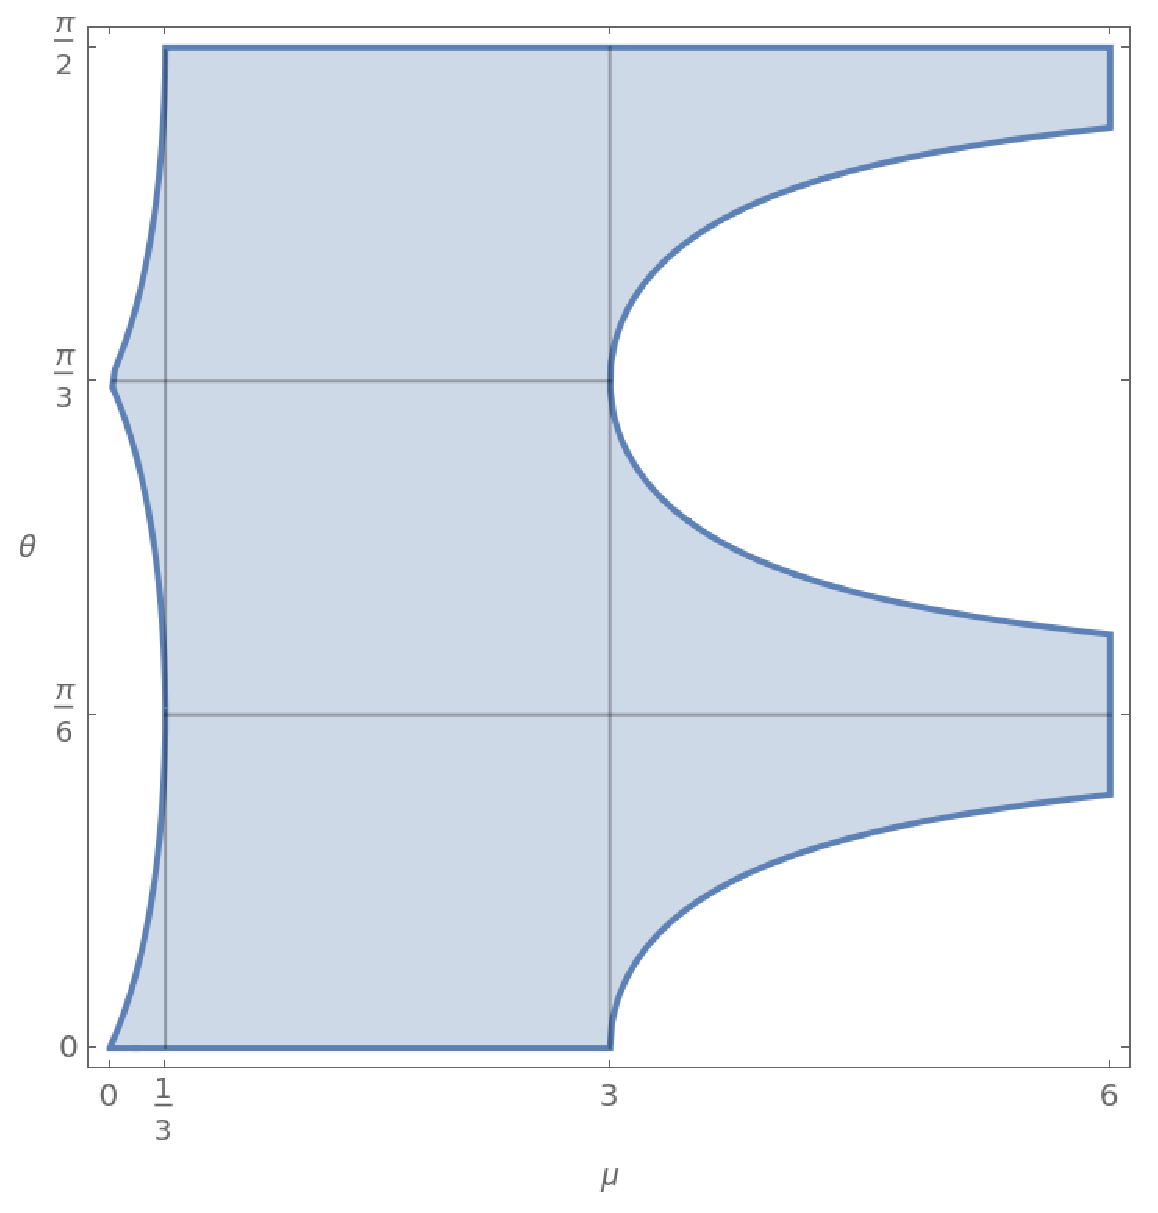
\includegraphics[width=0.5\linewidth]{mu-theta-feasibility-plot-notitle}\caption{$\mu-\theta$ Feasibility Plot}
\end{figure}


\section{Research Problem}

We seek solutions of
\begin{equation}
H_{V}\frac{\tilde{y}_{i}}{\tilde{m}_{R}}=\sum_{k\in N_{i}}\frac{2Q_{R}\left(\left|\tilde{y}_{k}-\tilde{y}_{i}\right|\right)}{\left\Vert u_{R}\right\Vert _{L^{2}}^{2}R^{4}\left|\tilde{y}_{k}-\tilde{y}_{i}\right|}\cdot\frac{\tilde{y}_{k}-\tilde{y}_{i}}{\tilde{m}_{R}}\label{eq:reduced-system}
\end{equation}
such that $\frac{\tilde{y}_{i}}{\tilde{m}_{R}}\xrightarrow[R\searrow0]{}y_{i}$
and 
\[
\frac{2Q_{R}\left(\left|\tilde{y}_{k}-\tilde{y}_{i}\right|\right)}{\left\Vert u_{R}\right\Vert _{L^{2}}^{2}R^{4}\left|\tilde{y}_{k}-\tilde{y}_{i}\right|}\xrightarrow[R\searrow0]{}\tilde{\alpha}_{ki}.
\]
We write $\tilde{y}_{i}=\tilde{m}_{R}y_{i}+\delta y_{i}$ (such that
$\frac{\delta y_{i}}{\tilde{m}_{R}}\xrightarrow[R\searrow0]{}0$),
$\delta y_{i}\in\text{span}\left\{ \boldsymbol{r_{1}},\boldsymbol{r_{2}}\right\} \forall i=\overline{1,3}$,
$R>0$. Define
\begin{equation}
F_{i}\left(\delta y,R\right)=H_{V}y_{i}+H_{V}\frac{\delta y_{i}}{\tilde{m}_{R}}-\sum_{k\in N_{i}}\frac{2Q_{R}\left(\left|\tilde{m}_{R}\left(y_{k}-y_{i}\right)+\delta y_{k}-\delta y_{i}\right|\right)}{\left\Vert u_{R}\right\Vert _{L^{2}}^{2}R^{4}\left|\tilde{m}_{R}\left(y_{k}-y_{i}\right)+\delta y_{k}-\delta y_{i}\right|}\left(y_{k}-y_{i}+\frac{\delta y_{k}-\delta y_{i}}{\tilde{m}_{R}}\right),\label{eq:Fi-definition}
\end{equation}
and extend $F_{i}$ at $R=0$ by continuity
\begin{equation}
F_{i}\left(\delta y,0\right)=H_{V}y_{i}-\sum_{k\in N_{i}}\underbrace{e^{-\left\langle y_{k}-y_{i},\delta y_{k}-\delta y_{i}\right\rangle }\chi}_{\alpha_{ki}\,=\,\tilde{\alpha}_{ki}\chi}\left(y_{k}-y_{i}\right),\label{eq:Fi-at-zero}
\end{equation}
with derivative along a vector $w\in\text{span}\left\{ \boldsymbol{r_{1}},\boldsymbol{r_{2}}\right\} $
\begin{equation}
D_{\delta y}F_{i}\left(\delta y,0\right)\left[w\right]=\sum_{k\in N_{i}}\left\langle w_{k}-w_{i},y_{k}-y_{i}\right\rangle e^{-\left\langle y_{k}-y_{i},\delta y_{k}-\delta y_{i}\right\rangle }\chi\left(y_{k}-y_{i}\right).\label{eq:Fi-derivative}
\end{equation}
With the ultimate goal of utilizing the implicit function theorem
(IFT) we must start with a solution of 
\begin{equation}
F_{i}\left(\delta y,0\right)=0\quad\forall i=\overline{1,3}\label{eq:Fi-system}
\end{equation}

\begin{claim}
$\delta y^{0}=\left(\delta y_{1}^{0},\delta y_{2}^{0},\delta y_{3}^{0}\right)$,
$\delta y_{1}^{0}=-\gamma\boldsymbol{r_{2}}$, $\delta y_{2,3}^{0}=\mp\beta\boldsymbol{r_{1}}+\frac{\gamma}{2}\boldsymbol{r_{2}}$,
with $\beta=\frac{1}{2}\ln\left(\frac{\alpha_{12}}{\alpha_{23}}\right)$,
$\gamma=\frac{2\beta}{3\sqrt{3}}$ solves (\ref{eq:Fi-system}).
\end{claim}
\begin{proof}
Plugging the given ansatz into (\ref{eq:Fi-system}) we obtain
\[
\begin{cases}
F_{1}= & H_{V}y_{1}-\left(e^{-\left\langle y_{2}-y_{1},\delta y_{2}-\delta y_{1}\right\rangle }\left(y_{2}-y_{1}\right)+e^{-\left\langle y_{3}-y_{1},\delta y_{3}-\delta y_{1}\right\rangle }\left(y_{3}-y_{1}\right)\right)\chi\\
F_{2}= & H_{V}y_{2}-\left(e^{-\left\langle y_{1}-y_{2},\delta y_{1}-\delta y_{2}\right\rangle }\left(y_{1}-y_{2}\right)+e^{-\left\langle y_{3}-y_{2},\delta y_{3}-\delta y_{2}\right\rangle }\left(y_{3}-y_{2}\right)\right)\chi\\
F_{3}= & H_{V}y_{3}-\left(e^{-\left\langle y_{1}-y_{3},\delta y_{1}-\delta y_{3}\right\rangle }\left(y_{1}-y_{3}\right)+e^{-\left\langle y_{2}-y_{3},\delta y_{2}-\delta y_{3}\right\rangle }\left(y_{2}-y_{3}\right)\right)\chi
\end{cases}
\]
With $\tilde{\alpha}_{ki}=e^{-\left\langle y_{k}-y_{i},\delta y_{k}-\delta y_{i}\right\rangle }\Rightarrow\tilde{\alpha}_{ki}=\tilde{\alpha}_{ik}$,
we find $\tilde{\alpha}_{12}=\tilde{\alpha}_{21}=\tilde{\alpha}_{13}=\tilde{\alpha}_{31}=1$
and $\tilde{\alpha}_{23}=\tilde{\alpha}_{32}=\frac{\alpha_{23}}{\alpha_{12}}$.
For the equilateral triangle we know $\alpha_{12}=\alpha_{13}=-\frac{\lambda_{2}}{3}>\alpha_{23}=\frac{-\lambda_{1}+\frac{\lambda_{2}}{3}}{2}\Rightarrow\chi=\max\left\{ \alpha_{12},\alpha_{13},\alpha_{23}\right\} =\alpha_{12}=\alpha_{13}$
and $H_{V}=\begin{pmatrix}\lambda_{1} & 0\\
0 & \lambda_{2}
\end{pmatrix},y_{1}=\left(0,\frac{1}{\sqrt{3}}\right)^{\intercal},y_{2}=\left(-\frac{1}{2},-\frac{1}{2\sqrt{3}}\right)^{\intercal},y_{3}=\left(\frac{1}{2},-\frac{1}{2\sqrt{3}}\right)^{\intercal}$. Therefore 
\[
\begin{cases}
H_{V}y_{1}-\left(\tilde{\alpha}_{21}\left(y_{2}-y_{1}\right)+\tilde{\alpha}_{31}\left(y_{3}-y_{1}\right)\right)\chi & =0\\
H_{V}y_{2}-\left(\tilde{\alpha}_{12}\left(y_{1}-y_{2}\right)+\tilde{\alpha}_{32}\left(y_{3}-y_{2}\right)\right)\chi & =0\\
H_{V}y_{3}-\left(\tilde{\alpha}_{13}\left(y_{1}-y_{3}\right)+\tilde{\alpha}_{23}\left(y_{2}-y_{3}\right)\right)\chi & =0
\end{cases}\Rightarrow\begin{cases}
H_{V}y_{1}-\left(y_{2}-y_{1}+y_{3}-y_{1}\right)\chi & =0\\
H_{V}y_{2}-\left(y_{1}-y_{2}+\frac{\alpha_{23}}{\alpha_{12}}\left(y_{3}-y_{2}\right)\right)\chi & =0\\
H_{V}y_{3}-\left(y_{1}-y_{3}+\frac{\alpha_{23}}{\alpha_{12}}\left(y_{2}-y_{3}\right)\right)\chi & =0
\end{cases}
\]
\[
\Downarrow
\]
\[
\begin{cases}
\begin{pmatrix}0\\
\frac{\lambda_{2}}{\sqrt{3}}
\end{pmatrix}-\left[\begin{pmatrix}-\frac{1}{2}\\
-\frac{\sqrt{3}}{2}
\end{pmatrix}+\begin{pmatrix}\frac{1}{2}\\
-\frac{\sqrt{3}}{2}
\end{pmatrix}\right]\chi & =\boldsymbol{0}\\
\begin{pmatrix}-\frac{\lambda_{1}}{2}\\
-\frac{\lambda_{2}}{2\sqrt{3}}
\end{pmatrix}-\left[\begin{pmatrix}\frac{1}{2}\\
\frac{\sqrt{3}}{2}
\end{pmatrix}+\frac{\alpha_{23}}{\alpha_{12}}\begin{pmatrix}1\\
0
\end{pmatrix}\right]\chi & =\boldsymbol{0}\\
\begin{pmatrix}\frac{\lambda_{1}}{2}\\
-\frac{\lambda_{2}}{2\sqrt{3}}
\end{pmatrix}-\left[\begin{pmatrix}-\frac{1}{2}\\
\frac{\sqrt{3}}{2}
\end{pmatrix}+\frac{\alpha_{23}}{\alpha_{12}}\begin{pmatrix}-1\\
0
\end{pmatrix}\right]\chi & =\boldsymbol{0}
\end{cases}\Rightarrow\begin{cases}
\begin{pmatrix}0\\
\frac{\lambda_{2}}{\sqrt{3}}
\end{pmatrix}+\begin{pmatrix}0\\
\sqrt{3}\alpha_{12}
\end{pmatrix} & =\boldsymbol{0}\\
\begin{pmatrix}-\frac{\lambda_{1}}{2}\\
-\frac{\lambda_{2}}{2\sqrt{3}}
\end{pmatrix}-\begin{pmatrix}\frac{\alpha_{12}}{2}\\
\frac{\sqrt{3}\alpha_{12}}{2}
\end{pmatrix}-\begin{pmatrix}\alpha_{23}\\
0
\end{pmatrix} & =\boldsymbol{0}\\
\begin{pmatrix}\frac{\lambda_{1}}{2}\\
-\frac{\lambda_{2}}{2\sqrt{3}}
\end{pmatrix}-\begin{pmatrix}-\frac{\alpha_{12}}{2}\\
\frac{\sqrt{3}\alpha_{12}}{2}
\end{pmatrix}+\begin{pmatrix}\alpha_{23}\\
0
\end{pmatrix} & =\boldsymbol{0}
\end{cases}
\]
\[
\Downarrow
\]
\[
\begin{cases}
\begin{pmatrix}0\\
\frac{\lambda_{2}}{\sqrt{3}}
\end{pmatrix}+\begin{pmatrix}0\\
-\frac{\sqrt{3}\lambda_{2}}{3}
\end{pmatrix} & =\boldsymbol{0}\\
\begin{pmatrix}-\frac{\lambda_{1}}{2}\\
-\frac{\lambda_{2}}{2\sqrt{3}}
\end{pmatrix}-\begin{pmatrix}-\frac{\lambda_{2}}{6}\\
-\frac{\sqrt{3}\lambda_{2}}{6}
\end{pmatrix}-\begin{pmatrix}\frac{-\lambda_{1}+\frac{\lambda_{2}}{3}}{2}\\
0
\end{pmatrix} & =\boldsymbol{0}\\
\begin{pmatrix}\frac{\lambda_{1}}{2}\\
-\frac{\lambda_{2}}{2\sqrt{3}}
\end{pmatrix}-\begin{pmatrix}\frac{\lambda_{2}}{6}\\
-\frac{\sqrt{3}\lambda_{2}}{6}
\end{pmatrix}+\begin{pmatrix}\frac{-\lambda_{1}+\frac{\lambda_{2}}{3}}{2}\\
0
\end{pmatrix} & =\boldsymbol{0}
\end{cases}\Rightarrow\begin{cases}
\begin{pmatrix}0\\
\frac{\lambda_{2}}{\sqrt{3}}-\frac{\lambda_{2}}{\sqrt{3}}
\end{pmatrix} & =\boldsymbol{0}\\
\begin{pmatrix}\frac{\lambda_{1}}{2}-\frac{\lambda_{1}}{2}\\
\frac{\lambda_{2}}{2\sqrt{3}}-\frac{\lambda_{2}}{2\sqrt{3}}
\end{pmatrix} & =\boldsymbol{0}\\
\begin{pmatrix}\frac{\lambda_{1}}{2}-\frac{\lambda_{1}}{2}\\
\frac{\lambda_{2}}{2\sqrt{3}}-\frac{\lambda_{2}}{2\sqrt{3}}
\end{pmatrix} & =\boldsymbol{0}
\end{cases}\:\checkmark
\]
$\therefore\delta y^{0}$ as stated above solves (\ref{eq:Fi-system})
for the equilateral triangle.
\end{proof}
\begin{claim}
(\ref{eq:Fi-derivative}) has a nontrivial kernel $\left(w_{1},w_{2},w_{3}\right)$
so the IFT does not apply.
\end{claim}
\begin{proof}
Let 
\begin{align*}
\Omega & =\ker\left(D_{\delta y}F_{i}\left(\delta y^{0},0\right)\right)\\
 & =\text{span}\left\{ \left(w_{1},w_{2},w_{3}\right)\vert\left\langle w_{k}-w_{i},y_{k}-y_{i}\right\rangle =0\,\forall\,i\neq k\right\} 
\end{align*}
We can immediately see that $\Omega\supseteq\boldsymbol{0}$. Consider
the following
\begin{align*}
\Phi & =\sum_{i}w_{i}\cdot D_{\delta y}F_{i}\left(\delta y,0\right)\left[w\right]\\
 & =\sum_{i}w_{i}\cdot\sum_{k\in N_{i}}\left\langle w_{k}-w_{i},y_{k}-y_{i}\right\rangle \cdot\alpha_{ik}\left(y_{k}-y_{i}\right)\\
 & =\sum_{k,i\in N_{k,i}}\alpha_{ik}\left\langle w_{k}-w_{i},y_{k}-y_{i}\right\rangle \left\langle w_{i},y_{k}-y_{i}\right\rangle +\alpha_{ki}\left\langle w_{i}-w_{k},y_{i}-y_{k}\right\rangle \left\langle w_{k},y_{i}-y_{k}\right\rangle \\
 & =-\sum_{k,i\in N_{k,i}}\alpha_{ik}\left(\left\langle w_{k}-w_{i},y_{k}-y_{i}\right\rangle \right)^{2}
\end{align*}
It follows that
\[
w\in\Omega\Longrightarrow\Phi\equiv\boldsymbol{0}
\]
and 
\[
\alpha_{ik}\neq0\Longrightarrow\left\langle w_{k}-w_{i},y_{k}-y_{i}\right\rangle =0\,\forall\,i\neq k
\]
which is precisely the defining condition placed on $\Omega$. Thus
$\left\{ \left(w_{1},w_{2},w_{3}\right)|\left\langle w_{k}-w_{i},y_{k}-y_{i}\right\rangle =0\,\forall\,i\neq k\right\} \subseteq\Omega$,
therefore (\ref{eq:Fi-derivative}) has a nontrivial kernel. For example,
take all three vectors equal. (Let $v\in\mathbb{R}^{2}$ be any nonzero
vector and set

\[
w_{1}=w_{2}=w_{3}=v.
\]
Then $w_{k}-w_{i}=0$ for every pair $\left(i,k\right)$, hence $\left\langle w_{k}-w_{i},y_{k}-y_{i}\right\rangle =0$.
Therefore $\left(v,v,v\right)\in\Omega$. Because $v$ can be chosen
arbitrarily in $\mathbb{R}^{2}$, the kernel $\Omega$ contains at
least the $2-$dimensional subspace

\[
\left\{ \left(v,v,v\right)\mid v\in\mathbb{R}^{2}\right\} \subsetneq\left\{ 0\right\} ,
\]
which is nontrivial. In particular, $\Omega\neq\left\{ 0\right\} $.)
\end{proof}
Assume $\left(w_{1},w_{2},w_{3}\right)\in\Omega$. Consider
\begin{align*}
P_{w}F\left(\delta y,R\right) & =\sum_{i}w_{i}\cdot F_{i}\left(\delta y,R\right)\\
 & =\sum_{i}\left[\left\langle w_{i},H_{V}y_{i}\right\rangle +\left\langle w_{i},H_{V}\frac{\delta y_{i}}{\tilde{m}_{R}}\right\rangle -\sum_{k\in N_{i}}\left[\left\langle w_{i},\alpha_{ik}\left(R\right)\left(y_{k}-y_{i}\right)\right\rangle +\alpha_{ik}\left(R\right)\left\langle w_{i},\frac{\delta y_{k}-\delta y_{i}}{\tilde{m}_{R}}\right\rangle \right]\right]\\
 & =\frac{1}{\tilde{m}_{R}}\sum_{i}\left[\left\langle w_{i},H_{V}\delta y_{i}\right\rangle -\sum_{k\in N_{i}}\alpha_{ik}\left(R\right)\left\langle w_{i},\delta y_{k}-\delta y_{i}\right\rangle \right]\\
 & =\frac{1}{\tilde{m}_{R}}\sum_{i}\left\langle w_{i},H_{V}\delta y_{i}-\sum_{k\in N_{i}}\alpha_{ik}\left(R\right)\left(\delta y_{k}-\delta y_{i}\right)\right\rangle 
\end{align*}
we then multiply by $\tilde{m}_{R}$ and extend continuously to $R\to0$
via
\begin{align*}
P_{w}F\left(\delta y,0\right) & =\sum_{i}\left\langle w_{i},H_{V}\delta y_{i}-\sum_{k\in N_{i}}\alpha_{ik}\left(0\right)\left(\delta y_{k}-\delta y_{i}\right)\right\rangle 
\end{align*}
with $\alpha_{ik}\left(0\right)=e^{-\left\langle y_{k}-y_{i},\delta y_{k}-\delta y_{i}\right\rangle }\chi$.
Now consider $P_{\perp}F\left(\delta y^{0},0\right)$ and $P_{\parallel}F\left(\delta y^{0},0\right)$
where $\perp,\parallel$ are with respect to $\Omega$. We then have
\begin{align*}
D_{\delta y}P_{\perp}F\left(\delta y^{0},0\right)\left[\delta w\right] & =P_{\perp}\sum_{k\in N_{i}}\left\langle \delta w_{k}-\delta w_{i},y_{k}-y_{i}\right\rangle \alpha_{ik}\left(0\right)\left(y_{k}-y_{i}\right)\\
D_{\delta y}P_{\parallel}F\left(\delta y^{0},0\right)\left[\delta w\right] & =\sum_{i}\left\langle w_{i},H_{V}\delta w_{i}\right\rangle \\
 & +\sum_{i}\sum_{k\in N_{i}}\left[\left\langle w_{i},\alpha_{ki}\left(0\right)\left(\delta y_{k}^{0}-\delta y_{i}^{0}\right)\right\rangle \left\langle y_{k}-y_{i},\delta w_{k}-\delta w_{i}\right\rangle -\alpha_{ki}\left(0\right)\left\langle w_{i},\delta w_{k}-\delta w_{i}\right\rangle \right]
\end{align*}
For $\delta w\in\Gamma=\ker\left(D_{\delta y}P_{\perp}F\left(\delta y^{0},0\right)\oplus D_{\delta y}P_{\parallel}F\left(\delta y^{0},0\right)\right)\Rightarrow\delta w\in\Omega$
and 
\[
\sum_{i}\left\langle w_{i},H_{V}\delta w_{i}-\sum_{k\in N_{i}}\alpha_{ki}\left(0\right)\left\langle w_{i},\delta w_{k}-\delta w_{i}\right\rangle \right\rangle =0
\]
for all $w\in\Gamma$. Alternatively, $\delta w\in\Gamma$ if and
only if $\delta w\in\Omega$ and
\begin{align*}
P_{\delta w} & =H_{V}\delta w_{i}-\sum_{k\in N_{i}}\alpha_{ki}\left(0\right)\left(\delta w_{k}-\delta w_{i}\right)\\
\Omega^{\perp} & \ni\\
 & =\left\{ z\in\mathbb{R}^{2\times3}|\exists c_{ki}=c_{ik}|z_{i}=\sum_{k\in N_{i}}c_{ki}\left(y_{k}-y_{i}\right)\right\} 
\end{align*}

\begin{claim}
If we restrict $\delta y_{1}$ to be orthogonal to $\boldsymbol{r_{1}}$
and $\delta y_{3}-\delta y_{2}$ to be parallel to $\boldsymbol{r_{1}}$.
From $\sum_{i}F_{i}\left(\delta y,R\right)=0$ we can find $\delta y_{1}\left(R\right),\delta y_{2}\left(R\right),\delta y_{3}\left(R\right)$
that solve (\ref{eq:reduced-system}) and $\delta y_{1}\left(0\right)=\delta y_{1}^{0},\delta y_{2}\left(0\right)=\delta y_{2}^{0},\delta y_{3}\left(0\right)=\delta y_{3}^{0}$.
\end{claim}
\begin{proof}
Starting with $\sum_{i}F_{i}\left(\delta y,R\right)=0$
\begin{align*}
\sum_{i}F_{i}\left(\delta y,R\right) & =0\\
\sum_{i}H_{V}y_{i}+H_{V}\frac{\delta y_{i}}{\tilde{m}_{R}}-\sum_{k\in N_{i}}\frac{2Q_{R}\left(\left|\tilde{m}_{R}\left(y_{k}-y_{i}\right)+\delta y_{k}-\delta y_{i}\right|\right)}{\left\Vert u_{R}\right\Vert _{L^{2}}^{2}R^{4}\left|\tilde{m}_{R}\left(y_{k}-y_{i}\right)+\delta y_{k}-\delta y_{i}\right|}\left(y_{k}-y_{i}+\frac{\delta y_{k}-\delta y_{i}}{\tilde{m}_{R}}\right) & =\\
\sum_{i}H_{V}\left(\frac{\tilde{m}_{R}y_{i}+\delta y_{i}}{\tilde{m}_{R}}\right)-\sum_{k\in N_{i}}\frac{2Q_{R}\left(\left|\tilde{m}_{R}\left(y_{k}-y_{i}\right)+\delta y_{k}-\delta y_{i}\right|\right)}{\left\Vert u_{R}\right\Vert _{L^{2}}^{2}R^{4}\left|\tilde{m}_{R}\left(y_{k}-y_{i}\right)+\delta y_{k}-\delta y_{i}\right|}\left(\frac{\tilde{m}_{R}y_{k}-\tilde{m}_{R}y_{i}+\delta y_{k}-\delta y_{i}}{\tilde{m}_{R}}\right) & =\\
\sum_{i}H_{V}\frac{\tilde{y}_{i}}{\tilde{m}_{R}}-\sum_{k\in N_{i}}\frac{2Q_{R}\left(\left|\tilde{m}_{R}y_{k}+\delta y_{k}-\left(\tilde{m}_{R}y_{i}+\delta y_{i}\right)\right|\right)}{\left\Vert u_{R}\right\Vert _{L^{2}}^{2}R^{4}\left|\tilde{m}_{R}y_{k}+\delta y_{k}-\left(\tilde{m}_{R}y_{i}+\delta y_{i}\right)\right|}\left(\frac{\tilde{m}_{R}y_{k}+\delta y_{k}-\left(\tilde{m}_{R}y_{i}+\delta y_{i}\right)}{\tilde{m}_{R}}\right) & =\\
\sum_{i}H_{V}\frac{\tilde{y}_{i}}{\tilde{m}_{R}}-\sum_{k\in N_{i}}\frac{2Q_{R}\left(\left|\tilde{y}_{k}-\tilde{y}_{i}\right|\right)}{\left\Vert u_{R}\right\Vert _{L^{2}}^{2}R^{4}\left|\tilde{y}_{k}-\tilde{y}_{i}\right|}\cdot\frac{\tilde{y}_{k}-\tilde{y}_{i}}{\tilde{m}_{R}} & =\\
 & \Downarrow\\
H_{V}\frac{\tilde{y}_{i}}{\tilde{m}_{R}}-\sum_{k\in N_{i}}\frac{2Q_{R}\left(\left|\tilde{y}_{k}-\tilde{y}_{i}\right|\right)}{\left\Vert u_{R}\right\Vert _{L^{2}}^{2}R^{4}\left|\tilde{y}_{k}-\tilde{y}_{i}\right|}\cdot\frac{\tilde{y}_{k}-\tilde{y}_{i}}{\tilde{m}_{R}} & =0
\end{align*}
which is precisely (\ref{eq:reduced-system}), and since
\begin{align*}
H_{V}\frac{\tilde{y}_{i}}{\tilde{m}_{R}} & =\sum_{k\in N_{i}}\frac{2Q_{R}\left(\left|\tilde{y}_{k}-\tilde{y}_{i}\right|\right)}{\left\Vert u_{R}\right\Vert _{L^{2}}^{2}R^{4}\left|\tilde{y}_{k}-\tilde{y}_{i}\right|}\cdot\frac{\tilde{y}_{k}-\tilde{y}_{i}}{\tilde{m}_{R}}\\
 & \Downarrow\:\left(R\searrow0\right)\\
H_{V}y_{i} & =\sum_{k\in N_{i}}\alpha_{ki}\chi\left(y_{k}-y_{i}\right)
\end{align*}
has solutions (by construction) $\delta y_{i}^{0}$, we also can see
$\delta y_{i}\left(0\right)=\lim_{R\searrow0}\delta y_{i}\left(R\right)=\delta y_{i}^{0}$.
\end{proof}
More generally, $\left(\delta y_{1},\delta y_{2},\delta y_{3}\right)\perp\left(w_{1},w_{2},w_{3}\right)=w_{\text{rot}}\iff\delta y\in\left\{ w_{\text{rot}}\right\} ^{\perp}$.
$F_{i}\left(\delta y_{i},R\right)$ does not necessarily preserve
$\left\{ w_{\text{rot}}\right\} ^{\perp}$; however, $\left\{ w_{\text{rot}}\right\} ^{\perp}=P_{\perp_{\text{rot}}}F_{i}\left(\delta y_{i},R\right)=0$
has a unique solution. If $F_{i}\left(R_{w}\delta y_{i},R\right)=R_{w}F_{i}\left(\delta y_{i},R\right)$
for all $w\in\left[-\pi,\pi\right]$, then $F_{i}\left(R_{w}\delta y_{i},R\right)=0$
such that $F_{i}\left(\delta y_{i},R\right)\mapsto R_{w}F_{i}\left(\delta y_{i},R\right)$
(since $F_{i}\left(\delta y_{i},R\right)=0$).

\section{Conclusion}

The present work has carried out a detailed finite-dimensional analysis
of multi-peak ground-state solutions of the nonlinear Schr�dinger
equation $\left(-\Delta+V+E\right)\psi+\sigma\left|\psi\right|^{2p}\psi=0$
in the high-energy regime $E\to\infty$. Working within the rescaling
and concentration-compactness framework established by Kirr and Natarajan
\cite{KirrNatarajan2018}, we reduced the existence question to an
algebraic system $F_{i}\left(\delta y,R\right)=0$ governing the positions
of well-separated profiles near a non-degenerate critical point of
the potential $V$.

Our main contributions are threefold. First, we systematically classified
all admissible multi-peak configurations in the limiting system ($R=0$):
collinear arrangements along a single eigenvector of the Hessian $H_{V}$,
isosceles and equilateral triangular configurations in the plane spanned
by two eigenvectors, and (most significantly) equilateral configurations
possessing a continuous rotational degree of freedom $\theta$. For
the rotational case we derived explicit admissibility regions in $\left(\mu,\theta\right)$
parameter space, where $\mu=\left|\lambda_{2}\right|/\left|\lambda_{1}\right|$
is the eigenvalue ratio: all orientations are admissible when $\frac{1}{3}\leq\mu\leq3$,
with restricted angular windows otherwise (Table 3.1, Figure 3.1).

Second, we formulated the perturbation system $F_{i}\left(\delta y,R\right)=0$
that governs how the limiting configurations deform at finite energy
($R>0$), and constructed explicit solutions $\delta y^{0}$ at $R=0$
for the equilateral triangle (Claim 3). We then showed (Claim 4) that
the linearization $D_{\delta y}F_{i}\left(\delta y^{0},0\right)$
has a nontrivial kernel $\Omega$ containing at least the two-dimensional
subspace $\left\{ \left(v,v,v\right)\mid v\in\mathbb{R}^{2}\right\} $,
corresponding to simultaneous rigid translation of the entire peak
configuration. This kernel obstruction prevents a direct application
of the implicit function theorem to continue solutions from $R=0$
to $R>0$.

Third, we began the resolution of this obstruction by following the
iterative kernel decomposition methodology developed by Kirr and Natarajan
\cite{KirrNatarajan2018} at the PDE and Lyapunov-Schmidt levels.
In their framework, each kernel obstruction encountered during the
continuation of solution branches is resolved by identifying the symmetry
responsible for the degeneracy and modding it out: at the PDE level,
the kernel of the full linearization $D_{\psi}F\left(\psi_{E},E\right)$
generated by the $U\left(1\right)$ gauge symmetry $\psi\mapsto e^{i\theta}\psi$
is removed by restricting to real-valued solutions (Theorem 2.1 of
\cite{KirrNatarajan2018}), yielding unique continuation of solution
branches modulo rotations; at the Lyapunov-Schmidt level, the kernel
of the linearized operator $L_{+}$ generated by translational invariance
is absorbed into translations of the individual profiles via the decomposition
in Lemma 3.2 and Proposition 7.6 of \cite{KirrNatarajan2018}. In
an analogous fashion, we decomposed the reduced finite-dimensional
system into projections $P_{\perp}F$ and $P_{\parallel}F$ perpendicular
and parallel to the kernel $\Omega$, identified the joint kernel
$\Gamma=\ker\left(D_{\delta y}P_{\perp}F\oplus D_{\delta y}P_{\parallel}F\right)$,
and characterized $\Omega^{\perp}$ as the subspace of perturbations
expressible as linear combinations of the inter-peak displacement
vectors $y_{k}-y_{i}$. The key structural observation (Claim 5) is
that by imposing gauge-fixing constraints (restricting $\delta y_{1}\perp r_{1}$
and $\delta y_{3}-\delta y_{2}\parallel r_{1}$, which remove the
rotational degree of freedom from the solution space) the projected
system $P_{\mathrm{rot}}^{\perp}F_{i}\left(\delta y,R\right)=0$ is
expected to admit a unique solution branch, provided the rotational
equivariance $F_{i}\left(R_{\omega}\delta y,R\right)=R_{\omega}F_{i}\left(\delta y,R\right)$
holds, so that the full orbit of solutions is recovered from any single
representative.

\textbf{The present work leaves the completion of this program at
a precise juncture.} The concentration-compactness decomposition,
the Lyapunov--Schmidt reduction to the finite-dimensional system,
and the framework for reconnecting finite-dimensional solutions back
to exact PDE solutions are all established by \cite{KirrNatarajan2018}
--- in particular, Lemma 2 guarantees that once the peak positions
$\left(z_{1},\ldots,z_{M}\right)$ are determined, the remainder $h_{R}$
is uniquely recovered via the implicit function theorem in $H^{1}$.
What remains is to complete the finite-dimensional step itself. Specifically:
\begin{enumerate}
\item \textbf{Rigorous verification of rotational equivariance.} The argument
in Claim 5 rests on the equivariance relation $F_{i}\left(R_{\omega}\delta y,R\right)=R_{\omega}F_{i}\left(\delta y,R\right)$.
The interaction terms in $F_{i}$ depend on the Euclidean distances
$\left|y_{k}-y_{i}\right|$ and inner products $\left\langle y_{k}-y_{i},\delta y_{k}-\delta y_{i}\right\rangle $,
which are rotation-invariant. However, the Hessian term $H_{V}$ is
diagonal in the eigenvector basis with generically distinct eigenvalues
($\lambda_{1}\neq\lambda_{2}$ when $\mu\neq1$), so it does not commute
with arbitrary rotations. The equivariance must therefore be established
at the level of the full system $F_{i}$ (showing that the Hessian
and interaction terms transform compatibly) rather than term by term.
This is the most immediate remaining step.
\item \textbf{Invertibility on the constrained subspace.} After modding
out the rotational kernel, the implicit function theorem requires
that $D_{\delta y}P_{\text{rot}}^{\perp}F_{i}\left(\delta y^{0},0\right)$,
restricted to the gauge-fixed subspace $\left\{ \delta y_{1}\perp r_{1},\;\delta y_{3}-\delta y_{2}\parallel r_{1}\right\} $,
is an isomorphism. This amounts to verifying that no kernel directions
remain beyond those generated by translations and rotations (equivalently,
that $\dim\Gamma$ equals the dimension of the symmetry group acting
on the configuration). Explicit computation of the reduced linearization
matrix and its determinant for the equilateral triangle would complete
this step.
\item \textbf{Extension to the $\boldsymbol{\theta-}$dependent configurations.}
The kernel analysis in Section 4 was carried out for the equilateral
triangle at a fixed orientation. For configurations with a continuous
rotational parameter $\theta$, the kernel $\Omega$ may acquire additional
structure reflecting the $\theta-$dependence of the interaction coefficients
$\alpha_{12}\left(\theta\right)$, $\alpha_{13}\left(\theta\right)$,
$\alpha_{23}\left(\theta\right)$. The gauge-fixing procedure must
be adapted accordingly, and the admissibility constraints $\alpha_{ki}\geq0$
derived in Section 3 must be shown to persist under the perturbation
$\delta y$.
\end{enumerate}
Once these finite-dimensional steps are completed, the existing Lyapunov--Schmidt
machinery of \cite{KirrNatarajan2018} immediately lifts the solutions
to exact multi-peak ground states of the full PDE for all sufficiently
large energies $E$. Moreover, the stability properties of such states
are already largely understood within the existing framework: \cite{KirrNatarajan2018}
showed that multi-profile branches with $m\geq2$ have $L_{+}$ with
at least two negative eigenvalues, which by the instability criterion
of \cite{GrillakisShatahStrauss1987} implies orbital instability.
Asymptotic stability of single-peak bound states was established by
\cite{KirrZarnescu2007,KirrZarnescu2009} via dispersive estimates
and the Fermi golden rule; adapting these techniques to the multi-peak
setting (where new spectral features may arise from the inter-peak
coupling) remains an open and interesting direction within the broader
program articulated by \cite{Kirr2016} of identifying all coherent
states, determining their stability, and describing the long-time
dynamics as convergence toward these states.

In summary, we have classified the admissible multi-peak geometries,
identified the kernel obstruction in the reduced system, and decomposed
the problem into components parallel and perpendicular to this kernel
following the iterative methodology of \cite{KirrNatarajan2018}.
The remaining task (verifying equivariance and invertibility on the
complement of the rotation-generated kernel) is a concrete, explicitly
computable finite-dimensional problem whose resolution would complete
the existence theory for multi-peak ground states at finite energy.

\section{Notation}

\subsection{Equation and Basic Parameters}
\begin{center}
\begin{table}[H]
\centering
\begin{tabular}{cc}
\toprule 
Symbol & Description\tabularnewline
\midrule
$\psi:\mathbb{R}^{n}\to\mathbb{C}$ & Solution of the nonlinear Schr�dinger equation\tabularnewline
$V:\mathbb{R}^{n}\to\mathbb{R}$ & External potential (encodes refractive index profile)\tabularnewline
$E\in\mathbb{R}^{+}\cup\left\{ 0\right\} $ & Energy parameter (propagation constant in optics)\tabularnewline
$\sigma\in\mathbb{R}^{+}$ & Nonlinearity coefficient (sign determines focusing/defocusing)\tabularnewline
$p$ & Nonlinear power exponent; $p=1$ corresponds to cubic (Kerr) nonlinearity\tabularnewline
$x_{0}$ & Non-degenerate critical point of $V$, i.e., $\nabla V\left(x_{0}\right)=0$
with $H_{V}\left(x_{0}\right)$ invertible\tabularnewline
\bottomrule
\end{tabular}

\caption{Notation - Equation and Basic Parameters}
\end{table}
\par\end{center}

\subsection{Scaling and Profile Functions}
\begin{center}
\begin{table}[H]
\centering
\begin{tabular}{cc}
\toprule 
Symbol & Description\tabularnewline
\midrule
$R=E^{-1/2}$ & Scaling parameter; $R\to0$ as $E\to\infty$\tabularnewline
$u_{E}\left(x\right)=E^{-\frac{1}{2p}}\psi_{E}\left(E^{-1/2}x\right)$ & Rescaled solution with $\left\Vert u_{E}\right\Vert _{H^{1}}$ uniformly
bounded\tabularnewline
$u_{R}$ & Profile function solving $\left(-\Delta+R^{2}V\left(x_{0}\right)+1\right)u+\sigma\left|u\right|^{2p}u=0$\tabularnewline
$M\in\mathbb{N}$ & Number of peaks in the multi-peak decomposition\tabularnewline
$z_{i}\left(R\right)$ & Position of the $i-$th peak center in rescaled coordinates\tabularnewline
$h_{R}$ & Remainder term: $u_{E}=\sum_{i=1}^{M}u_{R}\left(\cdot-z_{i}\right)+h_{R}$\tabularnewline
\bottomrule
\end{tabular}

\caption{Notation - Scaling and Profile Functions}

\end{table}
\par\end{center}

\subsection{Hessian and Spectral Properties}
\begin{center}
\begin{table}[H]
\centering
\begin{tabular}{cc}
\toprule 
Symbol & Description\tabularnewline
\midrule
$H_{V}=H_{V}\left(x_{0}\right)$ & Hessian matrix of $V$ at the critical point $x_{0}$\tabularnewline
$\lambda_{i}$ & Eigenvalue of $H_{V}$; assumed $\lambda_{i}<0$ for directions in
which peaks spread\tabularnewline
$\boldsymbol{r}_{i}$ & Unit eigenvector of $H_{V}$ associated with eigenvalue $\lambda_{i}$\tabularnewline
$\mu=\frac{\left|\lambda_{2}\right|}{\left|\lambda_{1}\right|}$ & Eigenvalue ratio; key parameter for admissibility constraints\tabularnewline
$U$ & Unstable manifold: $U=\text{span}\left\{ \boldsymbol{r}:H_{V}\boldsymbol{r}=\lambda\boldsymbol{r},\lambda<0\right\} $\tabularnewline
\bottomrule
\end{tabular}

\caption{Notation - Hessian and Spectral Properties}

\end{table}
\par\end{center}

\subsection{Bump Positions and Geometry}
\begin{center}
\begin{table}[H]
\centering
\begin{tabular}{cc}
\toprule 
Symbol & Description\tabularnewline
\midrule
$s_{i}=Rz_{i}-x_{0}$ & Displacement of $i-$th peak from critical point $x_{0}$\tabularnewline
$m_{R}$ & Minimum inter-peak distance: $m_{R}=\min_{i\neq j}\left|z_{i}\left(R\right)-z_{j}\left(R\right)\right|$\tabularnewline
$y_{i}=\lim_{R\to0}\frac{s_{i}}{Rm_{R}}$ & Limiting position vector of the $i-$th peak; satisfies $\left|y_{k}-y_{i}\right|=1$
for nearest neighbors\tabularnewline
$N_{i}$ & Set of nearest neighbors of peak $i$: $N_{i}=\left\{ k:\left|y_{k}-y_{i}\right|=1\right\} $\tabularnewline
$a,h$ & Geometric parameters for triangular configurations: $a$ = half-base,
$h$ = apex height\tabularnewline
\bottomrule
\end{tabular}

\caption{Notation - Bump Positions and Geometry}

\end{table}
\par\end{center}

\subsection{Interaction Functional and Coefficients}
\begin{center}
\begin{table}[H]
\centering
\begin{tabular}{cc}
\toprule 
Symbol & Description\tabularnewline
\midrule
$Q_{R}\left(z\right)$ & Interaction functional: $Q_{R}\left(z\right)=-\sigma\left\langle \partial_{\nicefrac{z}{\left|z\right|}}u_{R}\left(\cdot-z\right),u_{R}^{2p+1}\right\rangle $\tabularnewline
$\alpha_{ki}=\frac{Q_{R}\left(\left|z_{k}-z_{i}\right|\right)}{Q_{R}\left(m_{R}\right)}$ & Interaction coefficient between peaks $k$ and $i$; satisfies $0\leq\alpha_{ki}\leq1$\tabularnewline
$\tilde{\alpha}_{ki}=e^{-\left\langle y_{k}-y_{i},\delta y_{k}-\delta y_{i}\right\rangle }$ & Perturbed interaction coefficient at $R=0$\tabularnewline
$\chi=\frac{2Q_{R}\left(m_{R}\right)}{R^{4}m_{R}}$ & Overall interaction strength; $\chi>0$\tabularnewline
\bottomrule
\end{tabular}

\caption{Notation - Interaction Functional and Coefficients}

\end{table}
\par\end{center}

\subsection{Reduced System and Perturbations}
\begin{center}
\begin{table}[H]
\centering
\begin{tabular}{cc}
\toprule 
Symbol & Description\tabularnewline
\midrule
$\tilde{y}_{i}=\tilde{m}_{R}y_{i}+\delta y_{i}$ & Perturbed peak position; $\nicefrac{\delta y_{i}}{\tilde{m}_{R}}\to0$
as $R\to0$\tabularnewline
$\delta y_{i}\in\text{span}\left\{ \boldsymbol{r}_{1},\boldsymbol{r}_{2}\right\} $ & Perturbation of the $i-$th peak position\tabularnewline
$\delta y^{0}=\left(\delta y_{1}^{0},\delta y_{2}^{0},\delta y_{3}^{0}\right)$ & Explicit solution at $R=0$ with $\delta y_{1}^{0}=-\gamma\boldsymbol{r}_{2}$,
$\delta y_{2,3}^{0}=\mp\beta\boldsymbol{r}_{1}+\frac{\gamma}{2}\boldsymbol{r}_{2}$\tabularnewline
$\beta=\frac{1}{2}\ln\left(\frac{\alpha_{12}}{\alpha_{23}}\right)$ & Parameter in the explicit solution $\delta y^{0}$\tabularnewline
$\gamma=\frac{2\beta}{3\sqrt{3}}$ & Parameter in the explicit solution $\delta y^{0}$\tabularnewline
$F_{i}\left(\delta y,R\right)$ & \begin{cellvarwidth}[t]
\centering
Perturbation system governing peak positions.

$F_{i}\left(\delta y,0\right)=0$ characterizes limiting configurations
\end{cellvarwidth}\tabularnewline
\bottomrule
\end{tabular}

\caption{Notation - Reduced System and Perturbations}

\end{table}
\par\end{center}

\subsection{Kernel and Projections}
\begin{center}
\begin{table}[H]
\centering
\begin{tabular}{cc}
\toprule 
Symbol & Description\tabularnewline
\midrule
$\Omega$ & Kernel of $D_{\delta y}F_{i}\left(\delta y^{0},0\right)$; contains
$\left\{ \left(v,v,v\right):v\in\mathbb{R}^{2}\right\} $ (translations)\tabularnewline
$\Omega^{\perp}$ & Orthogonal complement: perturbations expressible as $z_{i}=\sum_{k\in N_{i}}c_{ki}\left(y_{k}-y_{i}\right)$\tabularnewline
$P_{\perp}F$, $P_{\parallel}F$ & Projections of $F$ perpendicular and parallel to the kernel $\Omega$\tabularnewline
$P_{w}F\left(\delta y,R\right)$ & Projection along $w\in\Omega$: $P_{w}F=\sum_{i}\left\langle w_{i},F_{i}\right\rangle $\tabularnewline
$\Gamma$ & Joint kernel: $\Gamma=\ker\left(D_{\delta y}P_{\perp}F\oplus D_{\delta y}P_{\parallel}F\right)$\tabularnewline
$P_{\delta w}$ & Linear operator acting on perturbations $\delta w_{i}$: $P_{\delta w}=H_{V}\delta w_{i}-\sum_{k\in N_{i}}\alpha_{ki}\left(0\right)\left(\delta w_{k}-\delta w_{i}\right)$\tabularnewline
$w_{\text{rot}}$ & Generator of the rotational kernel direction\tabularnewline
\bottomrule
\end{tabular}

\caption{Notation - Kernel and Projections}
\end{table}
\par\end{center}

\subsection{Rotations and Equivariance}
\begin{center}
\begin{table}[H]
\centering
\begin{tabular}{cc}
\toprule 
Symbol & Description\tabularnewline
\midrule
$\theta$ & Rotation angle; orientation of triangular configuration relative to
eigenvector basis\tabularnewline
$R\left(\theta\right)$ & 2D rotation matrix: $\begin{pmatrix}\cos\theta & -\sin\theta\\
\sin\theta & \cos\theta
\end{pmatrix}$\tabularnewline
$R^{-1}\left(\theta\right)=R\left(-\theta\right)$ & Inverse rotation matrix: $\begin{pmatrix}\cos\theta & \sin\theta\\
-\sin\theta & \cos\theta
\end{pmatrix}$\tabularnewline
$R_{\omega}$ & \begin{cellvarwidth}[t]
\centering
Rotation by angle $\omega$.

Used in equivariance condition $F_{i}\left(R_{\omega}\delta y,R\right)=R_{\omega}F_{i}\left(\delta y,R\right)$
\end{cellvarwidth}\tabularnewline
$y_{i}'=R^{-1}\left(\theta\right)y_{i}$ & Bump positions in the rotated (canonical) frame\tabularnewline
\bottomrule
\end{tabular}

\caption{Notation - Rotations and Equivariance}

\end{table}
\par\end{center}

\subsection{Admissibility Functions}
\begin{center}
\begin{table}[H]
\centering
\begin{tabular}{cc}
\toprule 
Symbol & Description\tabularnewline
\midrule
$\nu\left(\mu\right)=\frac{\mu+1}{2|\mu-1|}$ & \begin{cellvarwidth}[t]
\centering
Auxiliary function for admissibility.

Determines critical angle
\end{cellvarwidth}\tabularnewline
$\varphi\left(\mu\right)=\arccos\left(\nu\left(\mu\right)\right)$ & Critical angle function: $\varphi=\pi/3$ when $\nu\leq1/2$, $\varphi=0$
when $\nu\geq1$\tabularnewline
$\left(\mu,\theta\right)-$space & Parameter space for rotational equilateral configurations\tabularnewline
\bottomrule
\end{tabular}

\caption{Notation - Admissibility Functions}

\end{table}
\par\end{center}

\subsection{Inner Products and Norms}
\begin{center}
\begin{table}[H]
\centering
\begin{tabular}{cc}
\toprule 
Symbol & Description\tabularnewline
\midrule
$\left\langle \cdot,\cdot\right\rangle $ & Standard Euclidean inner product in $\mathbb{R}^{n}$ or $L^{2}$
inner product (context-dependent)\tabularnewline
$\left|\cdot\right|$ & Euclidean norm in $\mathbb{R}^{n}$\tabularnewline
$\left\Vert \cdot\right\Vert _{H^{1}}$ & Sobolev $H^{1}$ norm: $\left\Vert u\right\Vert _{H^{1}}^{2}=\left\Vert \nabla u\right\Vert _{L^{2}}^{2}+\left\Vert u\right\Vert _{L^{2}}^{2}$\tabularnewline
$\left\Vert \cdot\right\Vert _{L^{2}}$ & Standard $L^{2}$ norm\tabularnewline
$\perp$ & Orthogonality (with respect to $L^{2}$ or Euclidean inner product)\tabularnewline
\bottomrule
\end{tabular}

\caption{Notation - Inner Products and Norms}

\end{table}
\par\end{center}

\subsection{Linearization Operators}
\begin{center}
\begin{table}[H]
\centering
\begin{tabular}{cc}
\toprule 
Symbol & Description\tabularnewline
\midrule
$D_{\delta y}F_{i}$ & Fr�chet derivative of $F_{i}$ with respect to $\delta y$\tabularnewline
$D_{\delta y}F_{i}\left(\delta y^{0},0\right)\left[w\right]$ & Linearization at $\left(\delta y^{0},0\right)$ applied to direction
$w$\tabularnewline
$L_{+}$ & Linearized operator at the Lyapunov-Schmidt level. Kernel generated
by translational invariance\tabularnewline
$D_{\psi}F\left(\psi_{E},E\right)$ & Linearization of the full PDE at a solution $\psi_{E}$\tabularnewline
\bottomrule
\end{tabular}

\caption{Notation - Linearization Operators}

\end{table}
\par\end{center}

\begin{center}
%
\par\end{center}\pagebreak{}

\bibliographystyle{plain}
\bibliography{Research}


\end{document}
